\documentclass[11pt]{article}
\usepackage{booktabs}
\usepackage{natbib}
\usepackage{graphicx}
\usepackage{amsmath}
\usepackage{amssymb}
\usepackage{hyperref}
\usepackage{geometry}
\usepackage{cleveref}
\usepackage{todonotes}
% Sets off a heritable trait name (in small capitals) at its point of
% definition, marking the quantities that evolve under mutation and selection.
% Fixed or swept simulation parameters are not marked; they are referred to by
% their mathematical symbols. Restyle here to change every trait at once.
\newcommand{\trait}[1]{\textsc{#1}}
\title{The emergence and evolution of a referential code in
  populations of bee-like agents}
\author{Grzegorz Chrupała}
\date{}

\begin{document}

\maketitle

\begin{abstract}
\end{abstract}

\section{Introduction}
\label{sec:intro}
Communication in animal species takes many forms, from the chemical
signals of ants to the symbolic, compositional language of
humans. Each of these communication systems has its own idiosyncratic
properties. What ecological and evolutionary pressures shaped these
systems has been of substantial interest to biologists and cognitive
scientists.  In general, communication assumes some kind of shared code
between senders and receivers, and the emergence of such a code
requires a degree of alignment between these two roles.
Likewise, any change or modification to the code needs to be
coordinated between senders and receivers if the breakdown of
communication is to be avoided.

In many cases it is possible to think of a plausible pathway for the
coordinated emergence and development of a shared code, but a verbally
formulated scenario leaves many details underspecified and makes it
hard to be precise about the specific conditions that make code change
trajectories feasible. For this reason computational models of the
evolution of communication systems can provide insights which are hard to
obtain by other means. Such models have been used extensively to study
the emergence of communication and language (\Cref{sec:related}). In
this paper we model a transition of a particularly intriguing
communicative system in invertebrates: the waggle dance of honey bees.

Communication is referential when signals stand for entities or states in the
world rather than merely expressing the signaler's internal state. The
communicative code of \emph{Apis} species \cite{vonFrisch1967DanceLanguage} is a unique
referential system where food sites discovered by foraging scouts are indicated
to other members of the colony by means of a figure-of-eight dance whose axis
encodes the direction towards the food source, and whose duration stands for the distance
to it. In this study we focus on the signaling of direction, as its evolution illustrates
some interesting questions about coordination between participants in a communicative
system.
Different species of \emph{Apis} vary in the specific dance variant used to
encode the direction of the food patch: in species with exposed horizontal combs
(\emph{Apis florea} and \emph{Apis andreniformis}) the bees orient the axis of the
waggle dance directly towards the food patch. In other members of the \emph{Apis}
genus, combs are vertical and in some species also hidden in cavities. Such
combs make direct pointing impossible, and these species use gravity as a
reference point, and map the azimuth of the food patch relative to the sun onto
the angle of the waggle dance with respect to the vertical. \Cref{fig:waggle}
illustrates these two versions of the waggle dance.\footnote{This is a somewhat
simplified overview: in individual species there may be considerable behavioral
flexibility in how the dance is performed: e.g.\ in \textit{Apis mellifera}, sometimes
bees dance on a horizontal platform at the entrance to the beehive and in this case
they use direct pointing, even though this species generally employs the gravity
code \citep{Esch2012}.} 

The direct-pointing variant is iconic:
the form of the signal---the direction of the waggle axis---mirrors the direction
of the referent. The ancestral, direct-pointing dance has been characterized as 
an enactment of the foraging flight, in which the waggle run imitates the
departure  toward the food \citep{10.1242/jeb.142778}. The
gravity-referenced variant is more abstract, relying on an
indirect mapping of the sun's azimuth onto an angle measured from the vertical.
The waggle dance thus offers an opportunity to study  how a referential code
can shift from an iconic to a more abstract form, in a relatively simple system.

\begin{figure}
\centering
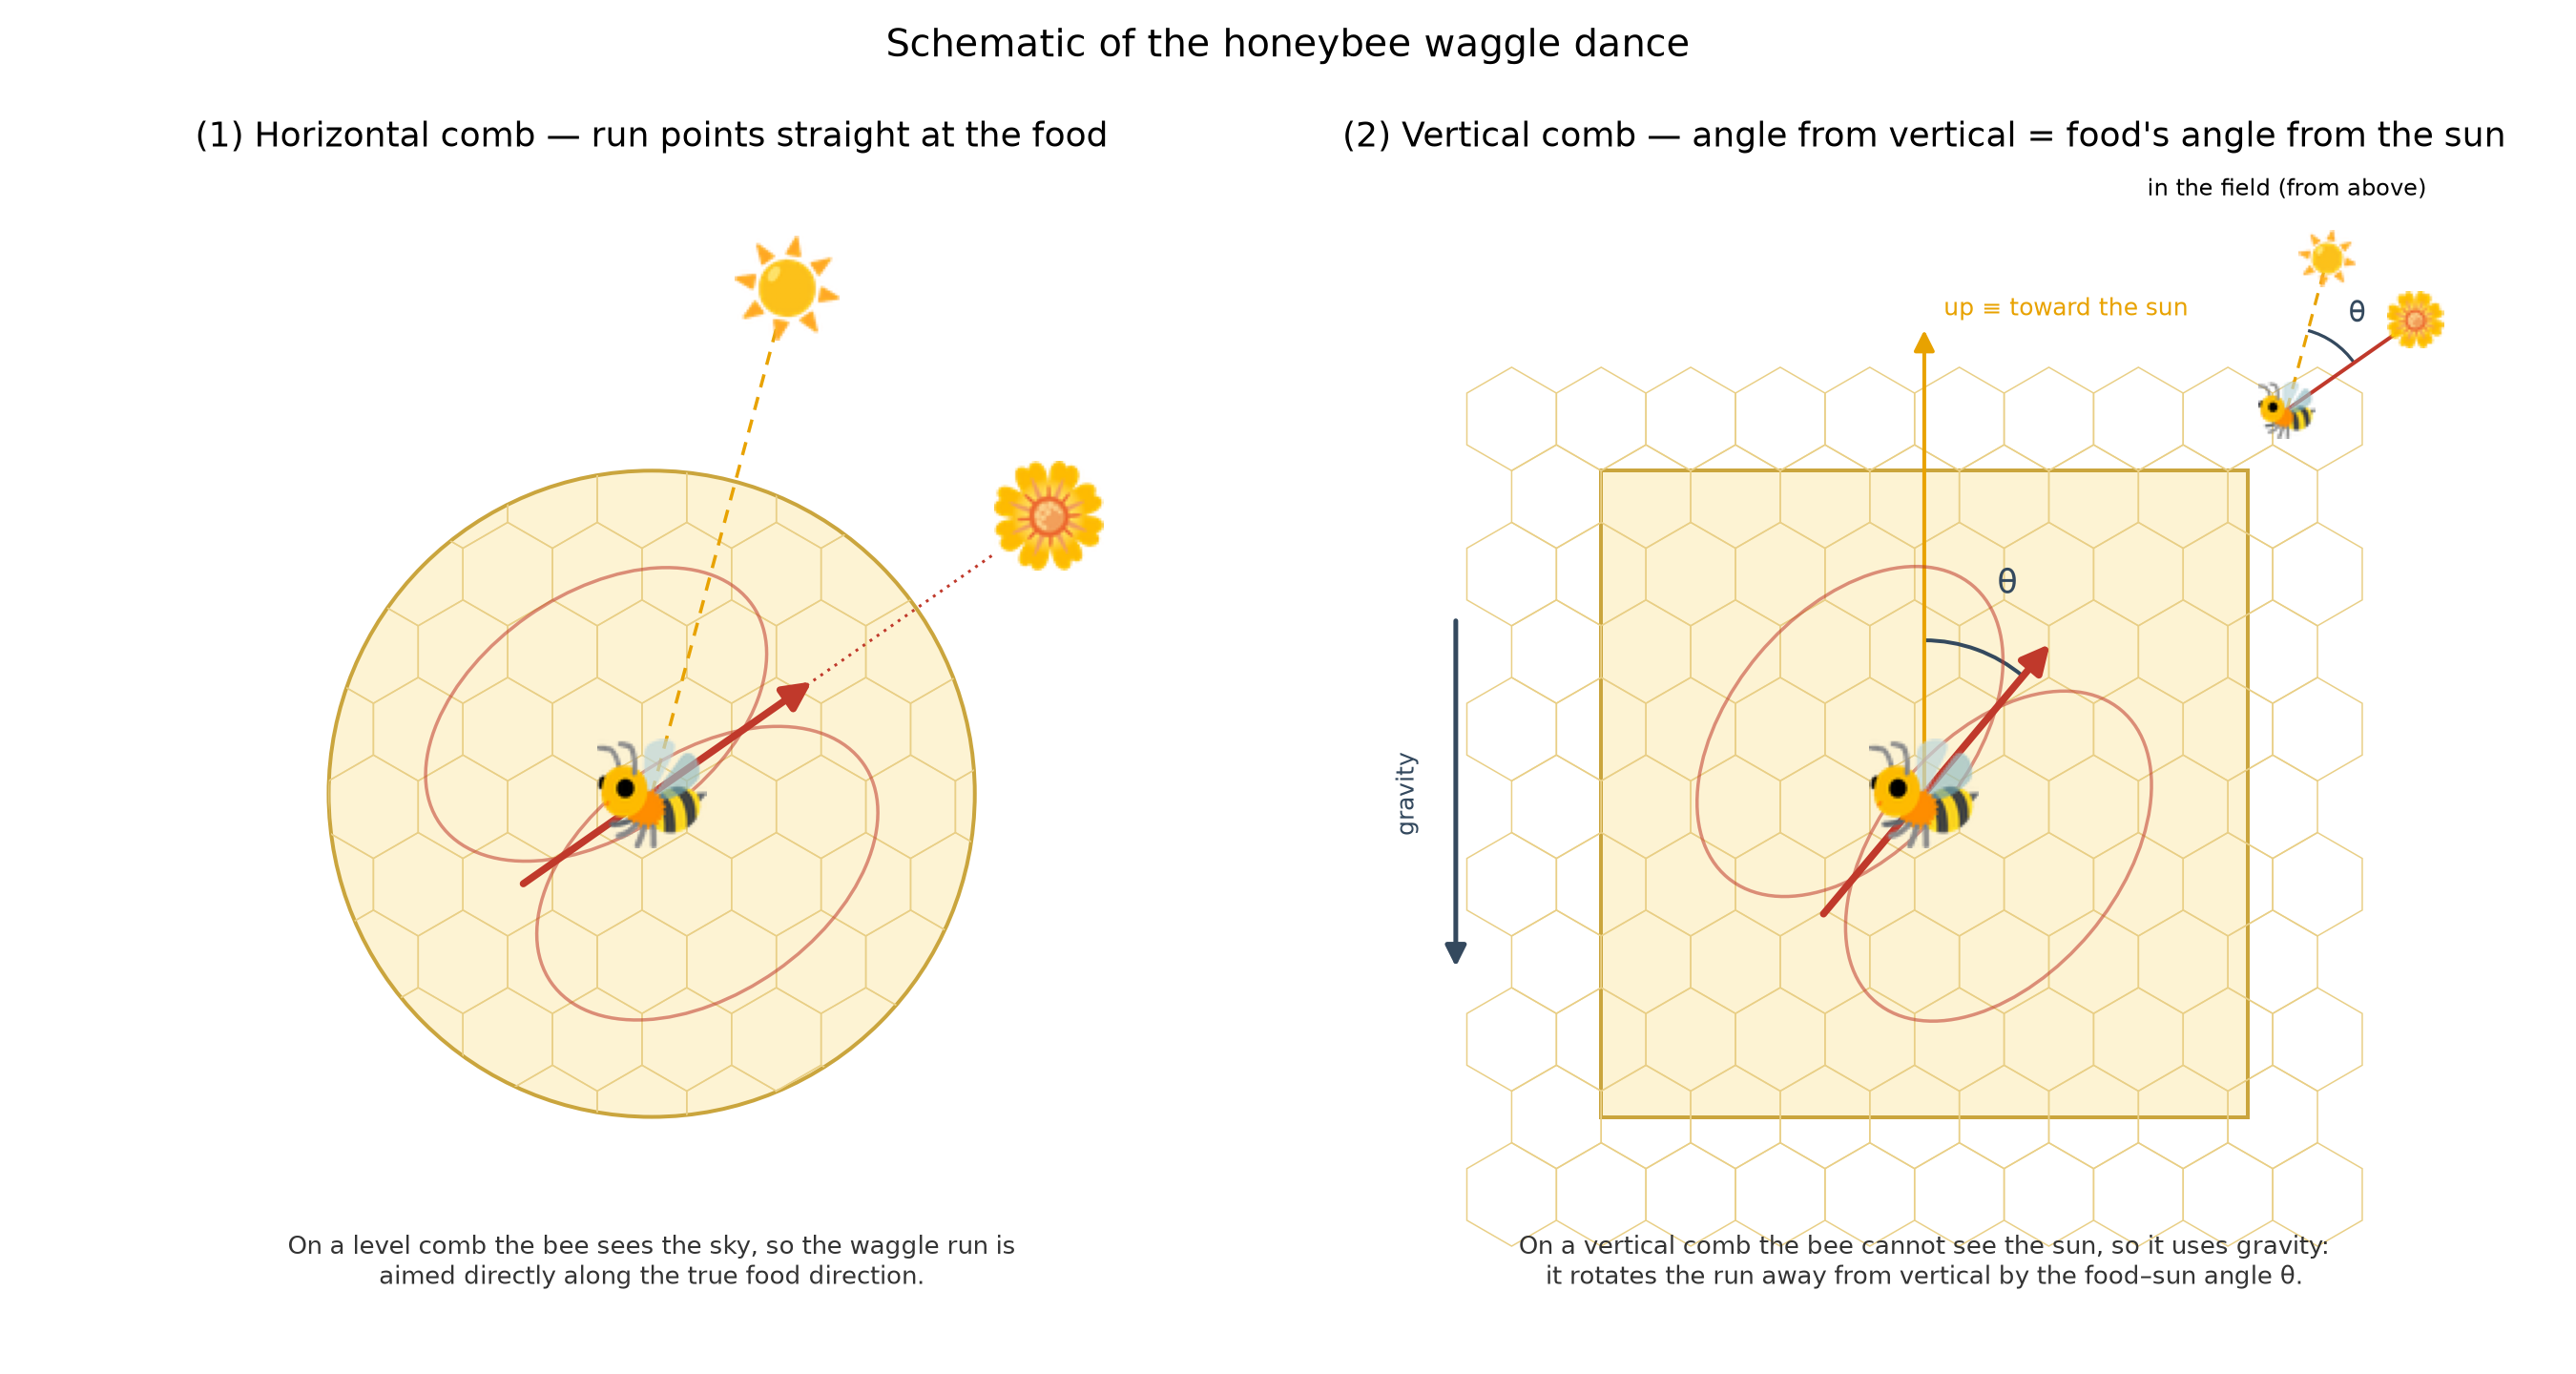
\includegraphics[width=0.8\textwidth]{figures/waggle_dance_schematic.png}   
\caption{The two variants of the honeybee waggle dance. On a horizontal,
exposed comb (left) the bee aims the straight waggle run
directly along the true direction to the food, which it can identify as being 
at a particular azimuth relative to the sun.  
On a vertical comb (right) the
bee cannot directly point at the food. Instead, it uses gravity as a reference: 
it maps the direction \textit{up} to the position of the sun, 
and it rotates the dance axis away from vertical by an
angle $\alpha$ equal to the food site's azimuth relative to the sun.
The figure-of-eight loops and the central waggle run are schematic and not to scale.}
\label{fig:waggle}  
\end{figure}

  
The distribution of comb orientation and waggle dance code throughout the \emph{Apis}
phylogeny (\Cref{fig:phylo}) suggests that the horizontal comb and direct
pointing are the ancestral state, extant in the stem \emph{Micrapis} subgenus.
Vertical
combs and the gravity-referenced code are derived traits, present in the other
two \emph{Apis} subgenera. Additionally, species within the \emph{Apis} sensu stricto
subgenus are cavity nesters. This pattern indicates that the
gravity code was linked to vertical combs and that cavity nesting is not
required for its emergence \citep{10.1242/jeb.142778}.

Nevertheless, the exact sequence and nature of evolutionary events that led to
the emergence of the gravity-based waggle dance is not known in detail. It is
also not clear how the transition from one version of the code to the other
could happen gradually, while maintaining communicative success at all stages,
and how this process interacted with the change in the orientation of
honeycombs. Because the code is shared, such a transition poses a coordination
problem: a change adopted by senders but not matched by the receivers'
interpretation, or the reverse, disrupts communication, so that intermediate
stages risk a loss of communicative success. A mechanistic account of this
transition has been proposed at the neural level: the central-complex circuitry
that represents the bee's directional heading (its own compass orientation) is not
tied to any particular spatial reference frame, so
a gravity reference could in principle substitute for the celestial one without a
dedicated switching mechanism \citep{10.1242/jeb.142778}. Such an account
addresses how an individual brain can support either version of the code, but
not how a population of senders and receivers stays coordinated while the shared
code itself evolves, which is the question we address.

\begin{figure}
    \centering
    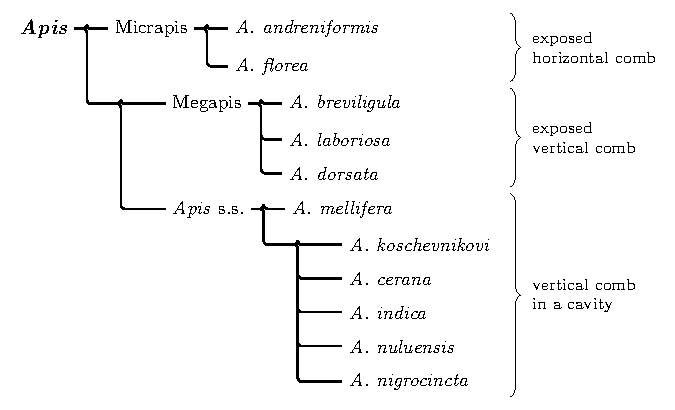
\includegraphics[width=0.8\textwidth]{figures/apis_phylogeny}
    \caption{A simplified illustration of the \emph{Apis} phylogeny, with the three
      subgenera \emph{Micrapis}, \emph{Megapis} and \emph{Apis} sensu stricto. Adapted from
      \citet{https://doi.org/10.1111/j.1365-3113.2009.00504.x}}
    \label{fig:phylo}
\end{figure}

The present study investigates this transition by means of a
computational model of evolving populations of bee-like agents. We
model selection at the level of colonies, and individual behavior at
the level of worker bees as colony members. We address two principal questions:
(i) under what ecological conditions a direct-pointing referential code
emerges and stabilizes, and (ii) which factors lead to a gradual
transition from this code to its gravity-referenced variant. Our aim is
not to reconstruct the precise historical sequence of these changes,
but to delineate the circumstances under which such a transition can
proceed without a breakdown of communication.

Our starting point is colonies with horizontal combs, which show some
heritable variation in traits controlling the inclination to direct
signaling and attending to signals. Here we show that:
communication via
direct pointing \emph{evolves readily when food is moderately hard to find by random
search alone}: i.e.\ when food sites are few in number but large, as well as when there 
are many small ones. It fails when food is too sparse to spark dances,
 or so abundant that it is found without signaling. 


In the second stage we introduce extrinsic evolutionary pressure for
vertical combs, which partially degrades the direct-pointing code while
making the gravity reference available. We show that in this scenario the
transition towards the gravity-referenced code is driven mainly by the \emph{
mutation rate} and the \emph{magnitude of the exogenous benefit of the vertical comb.}
Additionally the \emph{strength of the coupling between the signaling behavior
of senders and receivers} also plays a role, especially in the low-mutation-rate
regime.


The pattern of results from these simulations indicates that a basic
referential code based on an iconic, direct-pointing signal evolves
readily given favorable ecological conditions. On the other hand, the
transition from this basic ancestral system to the abstract code
based on gravity-referenced pointing requires the confluence of several key
favorable ecological and evolutionary factors; once these hold, however, the
transition proceeds reliably and without a breakdown of communication.

\section{Related work}
\label{sec:related}
The current study builds on several distinct strands of work. Firstly, it 
draws on research into the emergence and evolution of communication in 
artificial multi-agent systems, viewed as an abstract computational problem.
 Secondly, because our work is inspired by and grounded in real honeybee 
 societies, it also builds extensively on models and simulations of bee 
 communication. These studies are methodologically diverse, employing 
 agent-based models, neural models, evolutionary computation, or combinations
 thereof.

 \subsection{Communication in agent societies}
A long line of computational work has studied how communication systems can
emerge and stabilize in populations of interacting agents. The signaling game
introduced by \citet{lewis1969convention} provides the formal foundation for
much of this work, framing a convention of meaning as a solution to a recurring
coordination problem between a sender and a receiver. \citet{skyrms2010signals}
shows how such signaling conventions can arise without prior agreement through
evolutionary and reinforcement-learning dynamics. A distinct route emphasizes
cultural transmission: in the iterated-learning framework, linguistic structure
emerges as a code is repeatedly learned and reproduced across successive
generations of agents, without being built in \citep{smith2003iterated}. Related
formal work models how a protolanguage itself evolves under selection, showing
for instance how combining a small set of signals into words overcomes the error
limit that caps a simple signal repertoire \citep{nowak1999evolution}.
Agent-based models in this tradition have aimed to demonstrate that populations
playing repeated language games can self-organize shared, grounded vocabularies
and categories, a simulation tradition surveyed by \citet{wagner2003progress}.
More recently, deep multi-agent reinforcement learning has been used to show
that discrete communication protocols can emerge when agents are trained on
cooperative referential tasks \citep{lazaridou2017multi}. Subsequent work has
examined when such emergent codes become compositional and generalize to novel
meanings \citep{chaabouni2020compositionality}, and how communicative pressure
can drive neural agents towards attested language universals
\citep{lian2023communication}; see \citet{lazaridou2020emergent} for a review of
this line of research.

\subsection{Computational models of the waggle dance}
A venerable research tradition asks an ecological question: given that the dance
exists, \emph{when does it pay off}? The main tool here is the agent-based
foraging simulation. A colony of many simple forager agents follows fixed
behavioral rules. Dance recruitment is present as a switch, with recruits either
guided by a successful forager's spatial information or left to search on their
own, while the ecology (the density, quality, spread, and persistence of food
patches, and sometimes colony size) is varied across runs. The outcome of
interest is colony-level foraging performance: typically the net energy or
nectar collected. Importantly, these models represent neither evolution nor
within-lifetime learning: the communication strategy is fixed and the agents do
not adapt. What they model is the ecological cost-benefit accounting of a given
strategy: how a fixed colony fares, with recruitment versus without, in one
environment or another. Using such a model, \citet{dornhaus2006benefits} find
that recruitment benefits a colony mainly when resources are patchy, variable,
and hard to find, with the advantage depending on colony size, and
\citet{schurch2014dancing} show that the dance's long-term benefits can outweigh
its short-term costs. \citet{bailis2010positional} pose a more abstract version
of the same question, analyzing when positional communication beats reliance on
private information.  This body of work is the closest in spirit to our own
foraging payoff, but it holds the communication system constant and measures its
payoff in a fixed environment; it does not model the code itself as an evolving
trait.

More recently, the emergence itself of the bee communicative code has also been
investigated computationally. \citet{10.1371/journal.pcbi.1010487} treat
displaced communication as an evolutionary phenomenon: pairs of foraging agents,
each controlled by a continuous-time recurrent neural network, undergo
experimental evolution over tens of thousands of generations in a
one-dimensional circular arena where a receiver must reach one of several sites
a sender has perceived as holding food. Their central finding concerns how a
displaced signal arises. Although senders could in principle modulate  signal
amplitude, communication instead evolved from incidental, movement-derived cues
(the onset delay and duration of a sender's presence in the shared communication
zone), which were subsequently ritualized into signals. The more efficient
amplitude-based scheme evolved only when the cheaper cue was experimentally
suppressed. This model shares our evolutionary framing but selects at the level
of individual sender--receiver pairs rather than colonies, and it abstracts away
the geometry of the dance: the object of study is how any displaced signal
bootstraps from behavior, not how a specific directional code is structured.

\citet{siregar2026emergent} instead ask what internal representations and
channel properties allow a compositional, waggle-dance-like code to be
\emph{learned}. A single sender--receiver pair, implemented as graph neural
networks operating over map-like graphs of routes between the nest and candidate
sites, is trained by gradient descent on a referential game to transmit two
real-valued tokens identifying the food node. They ask whether the two tokens
factor into independent direction and distance components (compositionality),
how this depends on the overlap between the sender's and receiver's mental maps,
and whether constraining the channel to the kinematic range of a real dance
helps. They find that direction is readily encoded whereas direct distance is
not, that representational overlap is the main driver of compositionality, and
that channel constraints have only a small effect. This is a within-lifetime
study of representation and structure, with no population dynamics or selection.
In a similar vein, \citet{portegys2020morphognostic} has an individual agent
learn to both produce and follow dance-like movements that encode a nectar
location, again treating the dance as a code to be acquired within an
individual's lifetime rather than shaped by selection. The two differ in what is
left open: \citet{siregar2026emergent} let the code emerge from a referential
game and ask what structure results, whereas \citet{portegys2020morphognostic}
fixes the dance in advance and has a single agent learn to reproduce and respond
to it, studying acquisition of a known code rather than the emergence of its
structure.


\begin{table}
  \centering
  \small
  \begin{tabular}{@{}llll@{}}
    \toprule
    Approach & Code adapts by & Level & Question \\
    \midrule
    \multicolumn{4}{@{}l}{\emph{Communication in agent societies}}\\
    Signaling games and RL  & payoff dynamics       & population       & emergence \\
    Iterated learning       & transmission          & chain            & emergence \\
    Deep multi-agent RL     & learning              & pair             & emergence \\
    \addlinespace
    \multicolumn{4}{@{}l}{\emph{Models of the waggle dance}}\\
    Foraging simulations    & (fixed)               & colony           & payoff \\
    Evolved controllers     & evolution             & pair             & emergence \\
    Learned representations & learning              & individual/pair  & learnability \\
    \midrule
    \textbf{This work}      & evolution             & colony           & transition \\
    \bottomrule
  \end{tabular}
  \caption{Computational approaches to how a communicative code arises or
    changes, and where the present model sits among them. The columns give how
    the code adapts (if at all), the level it applies to, and the question each
    line of work asks. Rows are grouped into general models of communication and
    models specific to the waggle dance; each row is discussed and cited in the text.}
  \label{tab:routes}
\end{table}

Our study occupies a different point in this space (\Cref{tab:routes}). We model
the emergence and in particular the evolutionary \emph{transition} between two
forms of a referential code at the level of colonies, using a small set of
interpretable, heritable traits rather than opaque neural controllers. This lets
us treat costs, benefits, and comb geometry as explicit parameters and ask which
ecological and evolutionary conditions drive the shift from iconic direct
pointing to an abstract gravity-referenced code: a question about the conditions
and dynamics of a communicative transition that none of the prior work
addresses. 

\section{Method}
\label{sec:method}
Our  model is inspired by bee colonies and their waggle dance, but it is
simplified in many important ways, as our goal was not to model bee biology in
detail but rather investigate scenarios for the emergence and evolution of
referential communicative codes, while adopting the case of the waggle dance as a way
to ground the modeling in the real world and ensuring that it evolutionarily
plausible.

We model evolution at the level of colonies, and behavior at the level of
individual bee-like agents. This treatment is motivated by the reproductive and social
organization of real bee colonies, where workers are highly related and
sterile, and thus selection acts effectively on heritable colony-level traits
rather than on individual workers---this is the standard kin-selection rationale
for treating the honeybee colony as a superorganism
\citep{hamilton1964genetical,seeley1989superorganism}. We do not model sexual
reproduction: agent colonies reproduce without genetic input from other colonies. 
Colonies have a number of heritable
traits which are transmitted to offspring colonies subject to mutation, and
individual agents express these traits with some non-heritable individual
variation. In the interest of simplicity and focus, we model the waggle dance as only signaling 
the direction of a food site: our agents do not indicate distance.

\subsection{Colonies, workers, and traits}
\label{sec:traits}
We keep two kinds of quantity visually distinct throughout: a colony's heritable
traits, which evolve under mutation and selection and whose names we set in
\trait{small capitals}, and the model's fixed or swept simulation parameters,
which are chosen by the experimenter, referred to by their mathematical symbols,
and listed in \Cref{tab:fixed-params,tab:varied-params}. A colony is described
by a small set of heritable, real-valued traits, listed in full in
\Cref{tab:traits}. The prose here introduces the traits needed for the basic
horizontal-comb model (\Cref{sec:horizontal}); the additional traits and
geometry required for tilted combs are developed in \Cref{sec:vertical}.

\begin{table}
  \centering
  \small
  \begin{tabular}{@{}cll p{0.42\textwidth}@{}}
    \toprule
    Symbol & Name & Range & Role \\
    \midrule
    \multicolumn{4}{@{}l}{\emph{Behavioral (horizontal-comb model, \Cref{sec:horizontal})}}\\
    $b$      & \trait{directional bias}    & $[0,1]$ & sharpness of a dance about the food direction \\
    $a$      & \trait{receiver attention}  & $[0,1]$ & probability of following a dance rather than searching at random \\
    $p$      & \trait{dance propensity}    & $[0,1]$ & readiness to recruit others after a successful foraging attempt \\
    $\ell$   & \trait{foray distance}      & $[0,D]$ & mean outbound distance of a foray \\
    \addlinespace
    \multicolumn{4}{@{}l}{\emph{Nest and code choice (vertical transition, \Cref{sec:vertical})}}\\
    $\gamma$ & \trait{comb tilt}              & $[0,1]$ & comb inclination, $0$ horizontal to $1$ vertical \\
    $\phi$   & \trait{comb orientation}       & $[0,P)$ & compass heading the comb faces \\
    $t_s$    & \trait{sender transposition}   & $[0,1]$ & weight for the gravity code when producing a dance \\
    $t_r$    & \trait{receiver transposition} & $[0,1]$ & weight for the gravity code when interpreting a dance \\
    \bottomrule
  \end{tabular}
  \caption{The heritable, colony-level traits of the model. The first group
    governs behavior on a horizontal comb (\Cref{sec:traits,sec:horizontal}); the
    second adds the nest geometry and code-choice traits used in the vertical
    transition (\Cref{sec:vertical}). Workers express $b$, $a$, $p$, $t_s$, and
    $t_r$ with individual variation (\Cref{sec:traits}); $\ell$ varies 
    through the per-foray draw (\Cref{sec:environment}), and the nest traits
    $\gamma$ and $\phi$ are shared by all of a colony's workers. Here $D$ is the
    maximum search distance and $P$ the orientation period.}
  \label{tab:traits}
\end{table}

Four traits govern the behavior of a colony's workers. The \trait{directional
bias} $b$ controls how precisely a dance points; the \trait{receiver attention}
$a$ is the propensity to attend to a dance rather than to search at random; the
\trait{dance propensity} $p$ controls how readily a successful scout recruits
others to the patch it just found (\Cref{sec:foraging}); and the \trait{foray
distance} $\ell$ sets the mean outbound distance a worker travels on a foray. The first three are bounded to $[0,1]$ and the \trait{foray distance} to $[0,D]$,
where $D$ is the maximum search distance, a fixed model parameter (set to
$D = 6$ km in all our experiments).

Workers express the colony traits with non-heritable individual variation. A
worker $i$ realizes each trait $x \in \{b, a, p\}$ as
\begin{equation}
  x_i = \mathrm{clip}\bigl(x + \varepsilon_i\bigr), \qquad
  \varepsilon_i \sim \mathcal{N}(0, \eta^2),
\end{equation}
where $\eta$ is a fixed worker-variation scale and $\mathrm{clip}$ returns the
value to its admissible range. The \trait{foray distance} $\ell$ carries no separate
worker jitter: within-colony variation in how far workers travel arises instead
from the per-foray draw described in \Cref{sec:environment}. A colony thus
behaves as a noisy ensemble of workers sharing the same underlying genotype.

\subsection{Producing and interpreting signals}
\label{sec:signals}
On a horizontal comb the dance points directly at the food: this is the iconic,
direct-pointing code. A worker that has just foraged successfully at azimuth $\alpha$
produces a dance whose intended direction is $\alpha$ itself. The emitted signal is
drawn from a von Mises distribution centered on $\alpha$ with concentration
$\kappa = b_i\,\kappa_{\max}$, plus a small wrapped Gaussian dance noise. The von
Mises distribution is the circular analogue of a Gaussian: a signal $\psi$
centered on $\mu$ with concentration $\kappa$ has density
\begin{equation}
  f(\psi;\mu,\kappa) = \frac{\exp\bigl(\kappa\cos(\psi-\mu)\bigr)}{2\pi I_0(\kappa)},
\end{equation}
where $I_0$ is the modified Bessel function of order zero and $\kappa$ plays the
role of an inverse variance; here $\mu = \alpha$ and $\kappa = b_i\,\kappa_{\max}$.
The \trait{directional bias} $b$ therefore
controls the sharpness of the dance: a low bias leads to a near-uniform,
uninformative signal, while a high bias gives rise to a tightly concentrated one that
reliably indicates $\alpha$.

A worker that follows a dance reads its direction as a search direction, subject
to a small added interpretation noise. Communication is successful when this
recovered direction is close enough to a food site to lead the follower to it.

\subsection{Foraging environment}
\label{sec:environment}
A colony is evaluated over a fixed number of independent foraging episodes, and
its fitness is averaged over them (\Cref{sec:foraging}). Each episode draws a
fresh environment (\Cref{fig:environment}), with patch radii in meters and
distances from the nest in kilometers. The number of food sites is drawn from a
Poisson distribution with mean $n$, so episodes vary in how much food they offer.
 Each site is placed at an azimuth drawn uniformly around
the colony and at a distance drawn uniformly from $[d_{\min}, d_{\max}]$, and is
a physical circular disk whose radius is drawn independently from a
lognormal distribution with median $\rho_r$ and log-scale spread $\sigma_r$. A
forager finds the patch when its straight outbound path crosses the disk, so a
fixed patch subtends a smaller angle when farther from the nest, and distant
food demands more accurate dances. Each patch has value $v$ per visit and a finite
capacity limiting how many foragers it can supply before being exhausted;
capacity scales with the patch area, growing with the square of its radius, so
that larger patches hold proportionally more food while the per-visit value
stays fixed. In our
experiments $v = 1$, the median radius is $\rho_r = 150$ m with log-scale spread
$\sigma_r = 0.6$, a patch at the median radius has capacity $6$, and sites lie
between $d_{\min} = 0.75$ km and $d_{\max} = 6$ km.

The \trait{foray distance} trait $\ell$ (\Cref{sec:traits}) sets how far workers travel.
Each individual foray draws its own outbound length from a Gamma distribution
with mean $\ell$ and a fixed shape, capped at the maximum search distance $D$. The
per-foray draw is the source of within-colony variation in travel distance and
gives a realistic spread of short and long forays around the colony mean.

Each episode also fixes the position of the sun, which serves as the external
reference for the gravity-based code introduced in \Cref{sec:vertical}. The
sun's azimuth is drawn uniformly from an arc of width $\Delta_{\mathrm{sun}}$
centered on a fixed heading $\mu_{\mathrm{sun}}$ (in our experiments
$\mu_{\mathrm{sun}} = \pi/2$ and $\Delta_{\mathrm{sun}} = \pi$), so it is constant
within an episode but varies between episodes. We explain the role of this
variable sun azimuth in \Cref{sec:vertical}.
\begin{figure}
  \centering
    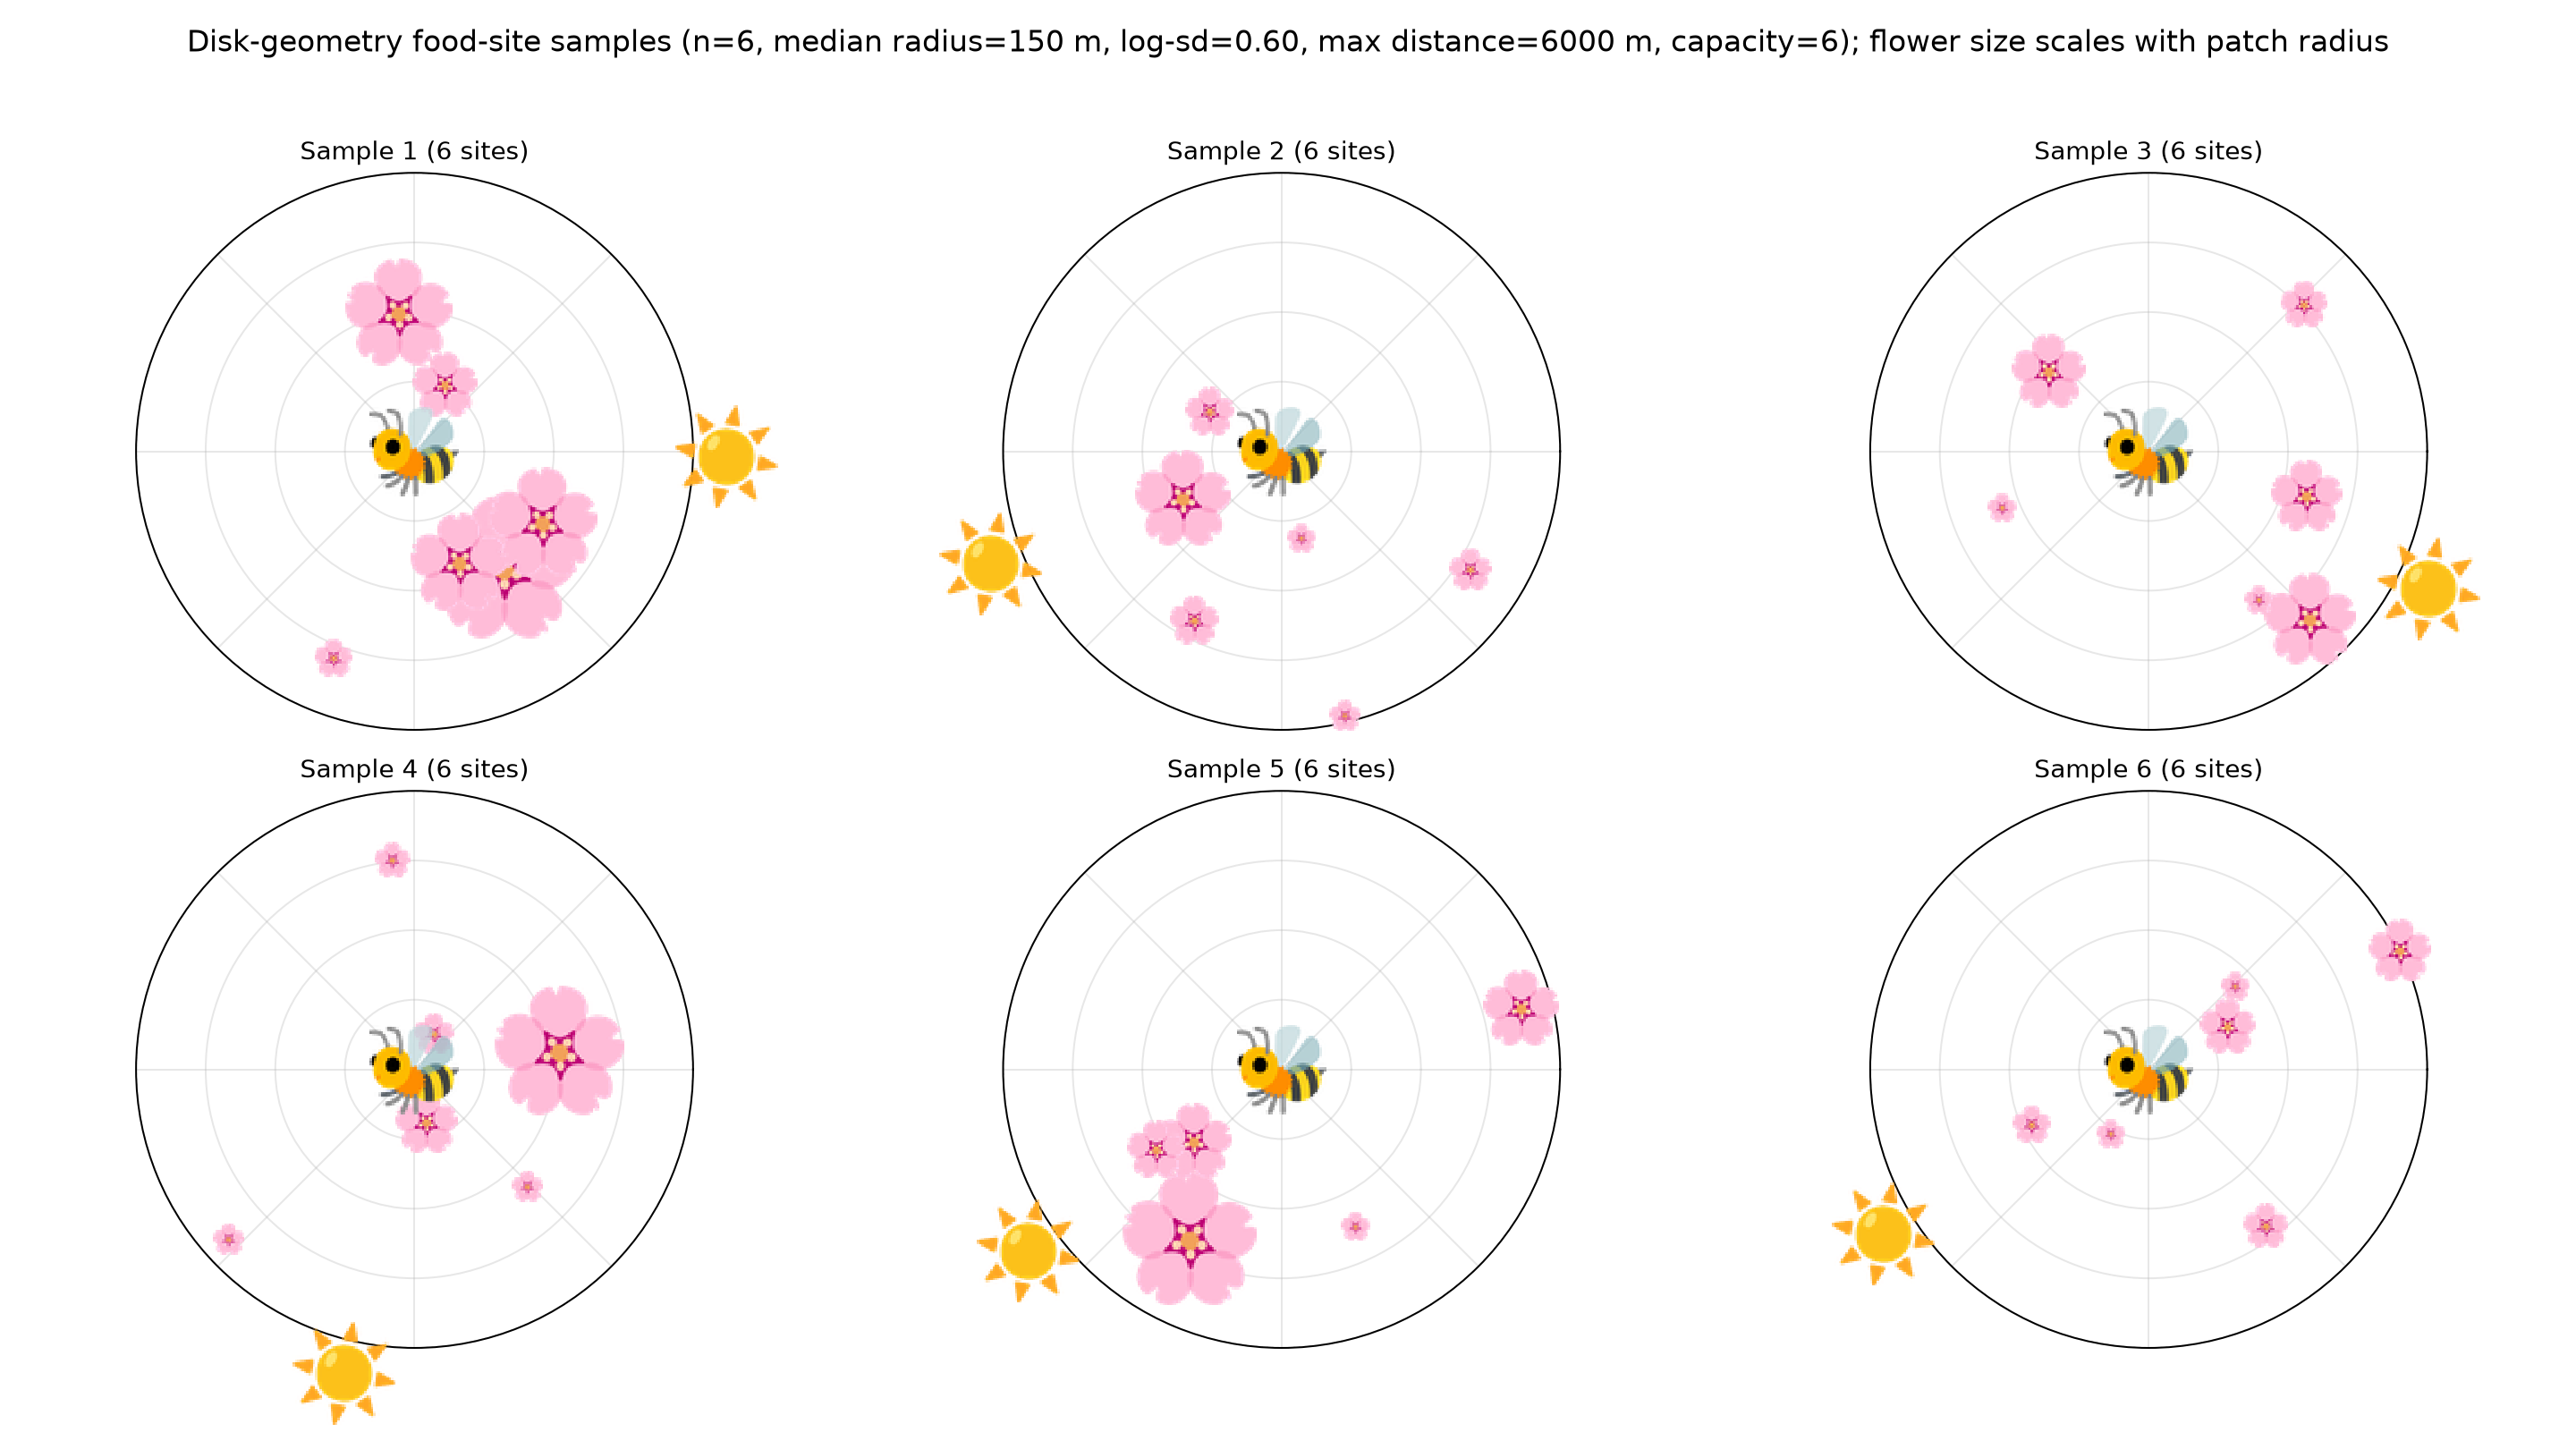
\includegraphics[width=0.8\textwidth]{figures/disk_food_samples.png}
    \caption{Six samples of the foraging environment. Each panel
      shows the colony (bee) at the centre, the food patches (flowers) at their
      drawn azimuths and distances, and the sun, which marks the external
      reference for the gravity-based code. Each patch is a physical disk, and
      the flower size scales with the sampled radius of the patch; radial rings mark
      distance from the colony in kilometers. Here the number of patches per episode
      is Poisson with mean $6$, so panels differ in how many patches they
      contain, with median radius $150$ m (lognormal, log-sd $0.6$), drawn out
      to a maximum distance of $6$ km.}
    \label{fig:environment}
\end{figure}

\subsection{Foraging and colony payoff}
\label{sec:foraging}
Within each episode (\Cref{sec:environment}) the colony makes a sequence of
foraging attempts. On each attempt a worker is drawn at random; if at least one
dance has already been performed in the current episode,
the worker follows a randomly chosen dance with probability equal to its
attention $a_i$, reading it out as a search direction, and otherwise searches in a
uniformly random direction. The worker then sets out along that direction on a
foray whose length is drawn as in \Cref{sec:environment} and enters the first
food patch on its path, among patches that still have remaining
capacity and lie within the foray length; if no patch is reached the attempt fails.

Payoff accrues per episode. A successful foraging attempt yields the patch value $v$, minus
a travel cost $c_{\mathrm{travel}}$ per unit of patch distance, and may prompt the worker to
perform a dance advertising the patch to later foragers. Recruitment is itself an
evolved decision: a successful scout dances with probability $1 - (1 - p_i)^{C}$,
where $p_i$ is its \trait{dance propensity} and $C$ is the patch's remaining capacity
after the visit, so an exhausted patch never leads to a dance and a scarcely
provisioned one rarely does. A dance, when performed, costs
$c_{\mathrm{base}} + c_{\mathrm{cue}}\,b_i$, growing with the precision of the
signal. A failed attempt costs travel proportional to the foray length it
travelled, and each act of attending to a dance incurs an attention cost $c_{\mathrm{att}}$.
Collecting these terms, an episode with successful attempts $S$ (each at distance
$r_k$), the subset $S_d \subseteq S$ of successes that produced a dance (each by a
worker with bias $b_k$), failed attempts $F$ (each with foray length $\ell_j$),
and $n_a$ dance-following attempts yields raw payoff
\begin{equation}
  \pi_{\mathrm{raw}} = \sum_{k \in S}\bigl(v - c_{\mathrm{travel}}\,r_k\bigr)
    - \sum_{k \in S_d}\bigl(c_{\mathrm{base}} + c_{\mathrm{cue}}\,b_k\bigr)
    - \sum_{j \in F} c_{\mathrm{travel}}\,\ell_j
    - c_{\mathrm{att}}\,n_a,
\end{equation}
where the dance-cost sum runs over $S_d$ because a success produces a dance only
when the recruitment decision is positive.
The scaled episode payoff is $\pi = (1 + B\gamma)\,\pi_{\mathrm{raw}}$, where
$\gamma$ is the \trait{comb tilt} and $B \ge 0$ the vertical-comb benefit; in the
horizontal model $\gamma = 0$, so the scaling is inert. We motivate its form in
\Cref{sec:transition}. A colony's fitness is its mean episode payoff (floored at a
small positive value).
For diagnostic purposes we also record a \emph{recruitment advantage}: the
difference between the success rate of workers that followed a dance and that of
contemporaneous workers that searched at random while dances were available. A
positive recruitment advantage indicates that the code is functioning, since
following a dance then beats searching blindly.

\subsection{Evolutionary dynamics}
\label{sec:evolution}
Evolution proceeds in non-overlapping generations over a fixed-size population of
colonies; there is no sexual reproduction. In each generation every colony is
evaluated, and the next generation is produced by repeated 
selection of parent colonies with a probability proportional to fitness. 
A selected colony's traits are copied subject to
mutation. Each trait is perturbed by an independent Gaussian step and then clipped to its
range. The step's standard deviation is a fixed fraction $\sigma_m$ of that
range: $\sigma_m$ for the traits on the unit interval, and $\sigma_m D$ for the
\trait{foray distance}, whose range is $[0,D]$. The workers of each offspring colony are then regenerated from its traits
as in \Cref{sec:traits}. The mutation rate $\sigma_m$ thus sets the pace of
evolutionary change.

\subsection{Horizontal comb}
\label{sec:horizontal}
The horizontal-comb model is exactly as described above: the comb is flat
and the only code available is direct pointing. We use it to
investigate the conditions under which a referential code emerges and stabilizes,
starting from an initial population with little communicative ability (low
\trait{directional bias} and low attention), so that early foragers signal weakly and
rarely attend to one another.

\subsection{Modeling code transition}
\label{sec:transition}
We ask how a colony can move from the direct-pointing code, available on a
horizontal comb, to the gravity-referenced code used on a vertical one. We do not
model why combs come to hang vertically; instead we impose an exogenous benefit
for vertical building through the payoff scaling $(1 + B\gamma)$
(\Cref{sec:foraging}), which rewards greater \trait{comb tilt} on its own, and ask
whether communication can survive as the comb tilts under that pressure. The
scaling is multiplicative because the advantages usually attributed to a vertical
comb are architectural,\footnote{A vertical comb carries cells on both faces of a
single sheet, whereas a horizontal one can open its cells only upward; and a comb
attached along its top edge is loaded in its own plane rather than in bending,
which wax tolerates better \citep{seeley1976nest,hepburn2014nests}.} and improve the return on what a colony
forages rather than paying a subsidy that arrives whether it forages or not. This
couples the two pressures, since tilt is then worth most to a colony that already
forages well, and therefore has a working direct code to lose. Because
\trait{comb tilt} is itself a trait that starts flat and evolves by small
mutational steps, a lineage passes through intermediate, partly tilted combs
rather than jumping from horizontal to vertical.

Those intermediate tilts are what make the transition non-trivial. As the comb
tilts, direct pointing degrades: projecting the food direction onto the sloping
surface foreshortens it in a bearing-dependent fashion, leaving less of the
direction in the surface to carry the signal. How faithfully the heading is
recovered depends on whether the receiver corrects for comb orientation. We thus
model two decoders (\Cref{sec:vertical}): a more biologically plausible
\emph{flatten} decoder which applies no such correction and is therefore biased
on a tilted comb, and an idealized \emph{unproject} decoder that corrects
exactly and serves as a bias-free reference against which to read the results of
\emph{flatten}.

Meanwhile, the growing tilt makes the
gravity-referenced code increasingly reliable, so a colony can in principle
switch codes as direct pointing weakens. We again model this switch as gradual,
through a blend of the two codes (\Cref{sec:vertical}).

\subsection{Dancing on a tilted comb}
\label{sec:vertical}
The tilted-comb model extends the horizontal one with the machinery for comb
tilt and the gravity-referenced code. It introduces two further
colony-level traits describing the nest: the \trait{comb tilt} $\gamma \in [0,1]$,
where $\gamma = 0$ is a horizontal comb and $\gamma = 1$ a vertical one, and the
\trait{comb orientation} $\phi$, the compass heading the comb faces. Like the
behavioral traits these are heritable and mutate by an independent Gaussian step
each generation, but they are
properties of the nest and so are shared by all of a colony's workers rather than
being expressed with individual variation. Because the orientation $\phi$ is an angle
defined on a circle of period $P$, its mutation step has standard deviation
$\sigma_m P$ rather than $\sigma_m$.

\paragraph{Comb geometry.}
The comb is a flat surface on which dances are performed, and its tilt determines
which reference directions a dance can use. We represent the comb by its unit
normal, the direction perpendicular to its face. When the comb is horizontal
this normal points straight up; as the comb tilts, the normal swings down toward
the horizon in the compass direction $\phi$, until on a vertical comb it lies
flat. Writing the tilt as a physical angle $\theta = \gamma\,\pi/2$ (so
$\theta = 0$ for a horizontal comb and $\theta = \pi/2$ for a vertical one), the
normal has eastward, northward, and upward components
\begin{equation}
  \mathbf{n} = \bigl(\,
    \underbrace{\sin\theta\cos\phi}_{\text{east}},\;
    \underbrace{\sin\theta\sin\phi}_{\text{north}},\;
    \underbrace{\cos\theta}_{\text{up}}
  \,\bigr).
\end{equation}
At $\theta = 0$ this reduces to $(0,0,1)$, pointing straight up, and at
$\theta = \pi/2$ it lies in the horizontal plane pointing along $\phi$.

\paragraph{The two codes.}
Both codes express the food direction as an angle in the comb surface; they
differ in the reference the angle is measured from and in how much of the
direction the surface can carry. In the \emph{direct} (iconic) code the worker
projects the world direction of the food, $\mathbf{f} = (\cos\alpha, \sin\alpha,
0)$, orthogonally onto the comb and dances along the resulting in-surface vector
$\mathbf{p}$ (\Cref{fig:direct-decode}).

\begin{figure}
  \centering
  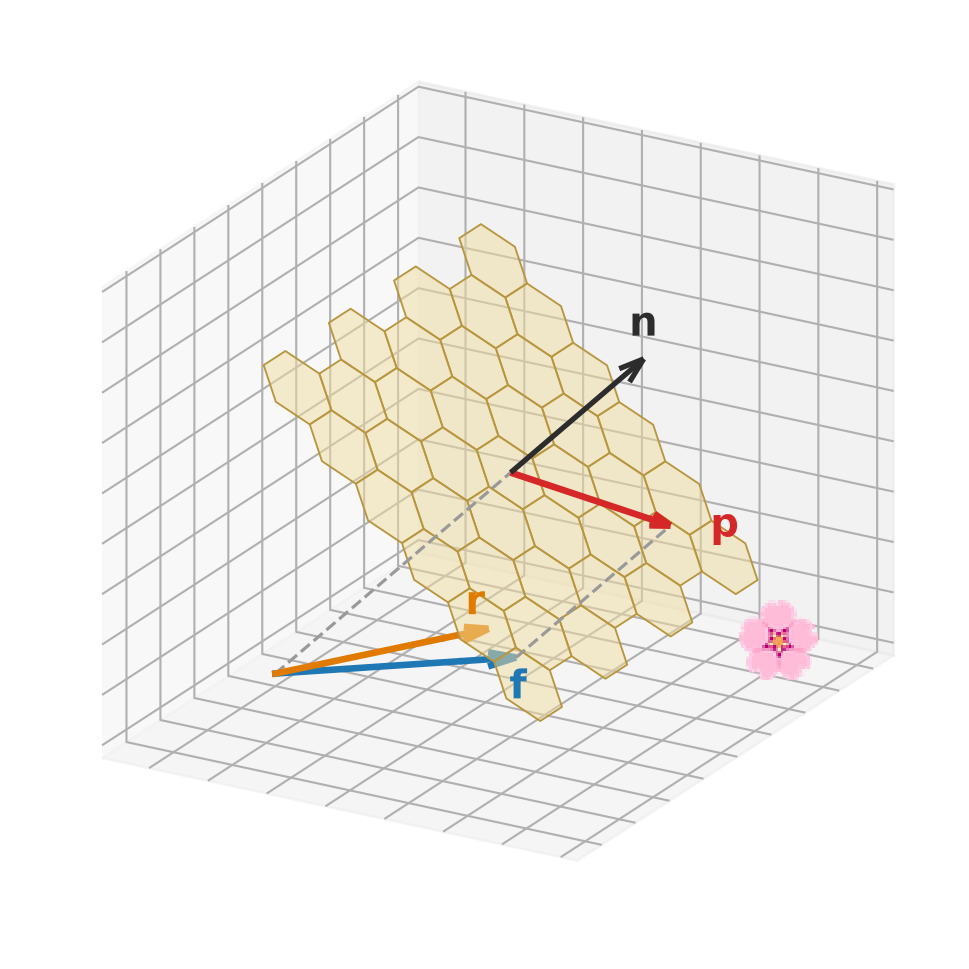
\includegraphics[width=0.6\textwidth]{figures/direct_decode.png}
  \caption{The direct code's projection and the flatten decode's bias. The
    tilted hexagonal comb and the world-horizontal plane (the grid) share the
    hive's east--north position. The food direction $\mathbf{f}$ (blue) lies
    in the world plane; its orthogonal projection onto the comb, $\mathbf{p}$
    (red), found by carrying its start and end points along the comb's
    normal $\mathbf{n}$ (black) until they meet the surface, shown by the
    dashed rays, has in-surface angle $\delta_\mathrm{dir}$, the encoded
    signal. Decoding that signal back to a world heading, the flatten variant
    recovers $\mathbf{r}$ (orange), which drifts off the true direction by a
    systematic angle on any tilted comb, whereas the unproject variant would
    recover $\mathbf{f}$ (blue) exactly. The flower marks the food site.}
  \label{fig:direct-decode}
\end{figure}

In the comb's orthonormal surface axes $\mathbf{e}_1, \mathbf{e}_2$, this
projection has coordinates $(p_1, p_2) = (\mathbf{e}_1\cdot\mathbf{f},\;
\mathbf{e}_2\cdot\mathbf{f})$, and the encoded signal is its angle
$\delta_{\mathrm{dir}} = \operatorname{atan2}(p_2,p_1)$. The code's
\emph{strength} is how much of the unit direction survives the projection,
$s_{\mathrm{dir}} = \lVert\mathbf{p}\rVert$. What the projection discards is the
part of $\mathbf{f}$ along the comb normal, $\mathbf{f}\cdot\mathbf{n} =
\sin\theta\cos(\alpha-\phi)$, leaving
\begin{equation}
  s_{\mathrm{dir}} = \sqrt{1 - \sin^2\theta\,\cos^2(\alpha-\phi)}.
\end{equation}
On a horizontal comb $s_{\mathrm{dir}} = 1$; that is the direction lies entirely within
the surface and is represented faithfully. As the comb tilts $s_{\mathrm{dir}}$
shrinks, reaching its minimum $\cos\theta$ for the food site in the direction the comb
faces ($\alpha = \phi$). Only on a fully vertical comb does this minimum fall to
zero: the facing direction then projects to nothing and its heading cannot be
recovered, while every other direction stays informative.

In the \emph{gravity-referenced} code the worker instead projects the vertical
direction $\mathbf{g} = (0,0,1)$ onto the comb to obtain an in-surface reference,
and encodes the food azimuth, measured relative to the sun, as an angle from that
reference. Its strength depends only on tilt, not on the bearing to the food site,
\begin{equation}
  s_{\mathrm{grav}} = \sin\theta = \sin(\gamma\,\pi/2),
\end{equation}
behaving oppositely to $s_{\mathrm{dir}}$: it is zero on a horizontal comb, where
gravity is perpendicular to the surface and gives no in-surface reference, and
grows to $1$ as the comb becomes vertical. The two trade off: a horizontal comb
supports only direct pointing, a vertical comb makes the gravity reference
available for every food direction, and at intermediate tilts both carry
information.

When code strength is below $1$, the direction it recovers is correspondingly
degraded, modeled as a circular interpolation between the true angle and a
uniformly random one with weight equal to the strength.

\paragraph{Decoding the direct code.}
The direct encoding is linear in the horizontal food vector:
$(p_1,p_2)^\top = M(\cos\alpha,\sin\alpha)^\top$, where $M$ is the $2\times 2$
matrix whose rows are the east--north parts of $\mathbf{e}_1,\mathbf{e}_2$, with
$\det M = \cos\theta$. Recovering the world heading exactly requires inverting
this map, and we model two receivers that differ in whether they do so
(\Cref{fig:direct-decode}). The inversion asks a lot of a receiver: it must know
\trait{comb tilt} and \trait{comb orientation}, and apply a correction that
varies with the direction danced. The uncorrected reading asks nothing, since the
dance is a direction in space and the food is on the ground: a receiver that
flies along the dance's compass bearing drops the vertical component simply by
flying. That reading is also exactly right on a horizontal comb (the ancestral
state), which is why we regard it as the more plausible of the two: it leaves the
ancestral rule unchanged, whereas the correction would have had no function to
select it before combs tilted.
\begin{description}
  \item[Unproject] The receiver applies $M^{-1}$, exactly inverting the
    encoding; since $\det M = \cos\theta > 0$ for $\theta < \pi/2$, the true
    heading is recovered without bias.
  \item[Flatten] The receiver reads the dance as a direction in space and drops
    its vertical component, taking the compass bearing of what is left. Where
    the sender projected the food direction onto the comb, the receiver projects
    the danced direction back onto the horizontal plane: a second projection
    rather than an undoing of the first, so the recovered heading $\mathbf{r}$
    is systematically biased on a tilted comb.\footnote{Formally, the receiver
    lifts $\delta$ to the in-surface vector $\cos\delta\,\mathbf{e}_1 +
    \sin\delta\,\mathbf{e}_2$ and keeps its east--north part, which applies
    $M^\top$ rather than $M^{-1}$. On a flat comb $M$ is a rotation, so the two
    coincide and the decodes are identical; they differ only once the comb
    tilts.}
\end{description}

The gravity code, by contrast, is always decoded by exact inversion:
the projected gravity reference is available to any receiver, so the sun-relative
food azimuth is read back directly.

\paragraph{Transposition and blending the codes.}
Which code a worker uses is governed by two further heritable behavioral traits,
the \trait{sender transposition} $t_s$ and \trait{receiver transposition} $t_r$
(both in $[0,1]$ and expressed with individual variation as in
\Cref{sec:traits}). These set how much weight a worker places on the
gravity-referenced code rather than the direct code when, respectively, producing
and interpreting a dance.\footnote{The alternative is a binary trait, with a
worker either pointing directly or referring to gravity and no blending in
between.We use graded weights because they let \trait{transposition} change by the
same small mutational steps as every other trait here, but they are the more
permissive of the two assumptions, and the transition we report should be read in
that light.}

Both roles blend the codes by the same rule. Given the angles
$\delta_{\mathrm{dir}}$ and $\delta_{\mathrm{grav}}$ the two codes assign, and a
transposition $t$, each angle is turned into a unit vector, scaled by its weight,
the two vectors are summed, and the blend is the heading of the resultant:
\begin{equation}
  \operatorname{blend}(\delta_{\mathrm{dir}}, \delta_{\mathrm{grav}};\, t)
    = \operatorname{atan2}\Bigl(\textstyle\sum_k w_k \sin\delta_k,\;
      \sum_k w_k \cos\delta_k\Bigr),
  \qquad k \in \{\mathrm{dir}, \mathrm{grav}\},
\end{equation}
where the weights combine the transposition with each channel's geometric
strength,
\begin{equation}
  w_{\mathrm{dir}} = (1 - t)\,s_{\mathrm{dir}}, \qquad
  w_{\mathrm{grav}} = t\,s_{\mathrm{grav}}.
\end{equation}
A sender blends the in-surface angles the two codes assign to the food just
visited, giving the intended dance direction
$\delta = \operatorname{blend}(\delta_{\mathrm{dir}}, \delta_{\mathrm{grav}};\,
t_{s,i})$, and emits a signal from a von Mises distribution about $\delta$ as in
\Cref{sec:signals}. A receiver decodes the observed signal under both codes and
blends the two recovered \emph{world} directions the same way, with $t_{r,i}$ in
place of $t_{s,i}$.

A worker with $t_i = 0$ therefore relies purely on direct pointing and one with
$t_i = 1$ purely on the gravity reference, while the strength factors ensure that
a code with no geometric support (such as the gravity code on a horizontal comb)
contributes nothing regardless of $t$. The geometric strength thus enters in two
distinct roles: it degrades the world direction each channel recovers,
interpolating it toward a uniformly random heading as described above, and it
scales that channel's weight in the blend, so a channel with weak geometric
support is at once less reliable and less relied upon.

Communication is accurate to the extent that senders and receivers weight the two
codes alike: the further $t_{r,i}$ sits from $t_{s,i}$, the more the receiver
reads the dance under a mix of references the sender did not use, and the larger
the resulting directional error. Alignment only matters where the codes disagree,
however, so on a horizontal comb, where $s_{\mathrm{grav}} = 0$ collapses both
blends onto the direct code, $t_r$ is free to drift.

The per-episode sun azimuth (\Cref{sec:environment}) matters through this
blending. Within an episode the sun is shared by every worker, so when a dancer
and follower both use the gravity code it enters encoding and decoding with
opposite sign and cancels, and where it falls does not matter. Because it varies
across episodes, however, a colony cannot treat it as a fixed offset: a strategy
that only partially commits to the gravity code leaves an uncancelled sun term,
so the shifting reference selects for genuine transposition rather than a stable
blend of the two codes.

\paragraph{Coupling of sender and receiver.}
A change of code pays off only to the extent that it is matched on the other
side, so the two traits may plausibly not mutate independently. We therefore
allow the mutations of $t_s$ and $t_r$ to be correlated, treating the strength of
the coupling as a parameter. Their mutational steps are drawn as a
correlated Gaussian pair whose sender--receiver coupling is the
correlation coefficient $\rho$,
\begin{equation}
  \Delta t_s = z_1, \qquad
  \Delta t_r = \rho\,z_1 + \sqrt{1-\rho^2}\;z_2, \qquad
  z_1, z_2 \sim \mathcal{N}(0, \sigma_m^2),
\end{equation}
which leaves the marginal mutation scale of each trait unchanged while tuning how
tightly the two co-vary. When $\rho$ is high, a mutation that pushes senders
toward the gravity code tends to push receivers by the same amount, so the two
sides of the code can shift in a coordinated fashion rather than drifting apart;
when $\rho = 0$ they evolve independently. The \trait{comb tilt} $\gamma$, held fixed at
$0$ in the horizontal model, is free to mutate in this version.
\paragraph{Selection for vertical combs.}
Finally, this version adds an extrinsic ecological pressure favoring vertical
combs, unrelated to communication. The raw episode payoff of \Cref{sec:foraging}
is scaled by a factor
\begin{equation}
  1 + B\,\gamma,
\end{equation}
where $B \ge 0$ is the magnitude of the vertical-comb benefit, so that taller
combs earn proportionally more. As $\gamma$ increases under this pressure the
direct channel degrades while the gravity channel becomes available, so
maintaining communicative success requires the population to migrate from the
direct to the gravity-referenced code. Because that shift must be matched on both
the sender and receiver sides, it constitutes the coordination problem of
interest, and we use this version to investigate how the benefit magnitude $B$,
the mutation rate $\sigma_m$, and the sender--receiver coupling $\rho$ govern
whether the transition proceeds without a breakdown of communication.

\section{Experimental setup}
We study the model of \Cref{sec:method} in two stages that mirror the two
questions of \Cref{sec:intro}. The first stage keeps the comb horizontal and asks
under what ecological conditions the direct-pointing code is worth maintaining
(\Cref{sec:setup-horizontal}). The second stage releases the comb and the
\trait{transposition} traits and asks under what conditions a population can migrate from
the direct to the gravity-referenced code as an extrinsic pressure tilts the comb
(\Cref{sec:setup-transition}). All experiments are run from configuration files
and fixed random seeds so that every reported run is reproducible.

\subsection{Fixed model parameters}
\label{sec:setup-fixed}
A core set of parameters is held fixed throughout, and only the ecological and
evolutionary parameters named below are varied. \Cref{tab:fixed-params} lists the
fixed values. The population contains $60$ colonies of $80$ workers each,
evolving for $120$ non-overlapping generations; each colony is evaluated over
$50$ independent foraging episodes of $12$ foraging attempts. Workers express
colony traits with variation scale $\eta = 0.08$ (\Cref{sec:traits}); dances are
emitted with maximum concentration $\kappa_{\max} = 14$ and production noise
$0.18$, and read with interpretation noise $0.12$ (\Cref{sec:signals}). All
lengths follow a fixed convention (distances in kilometers, patch radii in meters): the maximum search distance is $D = 6$ km and food
patches lie at distances in $[0.75, d_{\max}]$ km. Food patches are physical disks
whose radius is drawn from a lognormal of median $150$ m and log-scale spread
$0.6$; capacity scales with patch area from a base of $6$ loads at the median
radius, and the number of patches per episode is Poisson (\Cref{sec:environment}).
Each foray draws its outbound distance from a Gamma of shape $2$ with the colony's
evolved mean. Foraging carries a per-distance travel cost, a dance cost
$c_{\mathrm{base}} + c_{\mathrm{cue}}\,b_i$ with $c_{\mathrm{base}} = 0$ and
$c_{\mathrm{cue}} = 0.02$, and an attention cost $c_{\mathrm{att}} = 0.01$
(\Cref{sec:foraging}). The sun is drawn from an arc of width $\pi$ centered on
$\pi/2$, and the \trait{comb orientation} is treated as axially symmetric (period $\pi$).
Colonies start with little communicative ability: the initial \trait{directional bias} is
drawn from $\mathcal{U}(0,0.15)$, \trait{receiver attention} from $\mathcal{U}(0,0.25)$,
the \trait{foray distance} from $\mathcal{U}(0.15D, 0.45D)$, the \trait{dance propensity} from
$\mathcal{U}(0.8,1.0)$, and both \trait{transposition} traits start at $0$, so early
foragers signal weakly, rarely attend to one another, and use only direct
pointing.

\begin{table}
  \centering
  \begin{tabular}{lrl}
    \toprule
    Symbol / name & Value & Meaning \\
    \midrule
    colonies & $60$ & population size \\
    workers per colony & $80$ & ensemble size per colony \\
    generations & $120$ & evolutionary horizon (transition runs) \\
    episodes per colony & $50$ & foraging episodes averaged for fitness \\
    attempts per episode & $12$ & foraging attempts per episode \\
    $\eta$ & $0.08$ & worker-variation scale \\
    $\kappa_{\max}$ & $14$ & maximum dance concentration \\
    dance noise & $0.18$ & production noise (wrapped Gaussian) \\
    interpretation noise & $0.12$ & receiver decoding noise \\
    $D$ & $6$ & maximum search distance (km) \\
    $d_{\min}$ & $0.75$ & minimum food distance (km) \\
    $\rho_r$ & $150$ & median patch radius (m, lognormal) \\
    $\sigma_r$ & $0.6$ & patch-radius log-scale spread \\
    foray shape & $2$ & Gamma shape of per-foray distance \\
    $c_{\mathrm{base}},\,c_{\mathrm{cue}}$ & $0,\ 0.02$ & dance cost terms \\
    $c_{\mathrm{att}}$ & $0.01$ & attention cost \\
    $v$ & $1$ & food value \\
    $\mu_{\mathrm{sun}},\,\Delta_{\mathrm{sun}}$ & $\pi/2,\ \pi$ & sun arc center and width \\
    \bottomrule
  \end{tabular}
  \caption{Parameters held fixed across all experiments. Ecological parameters
    (food-site count, patch radius, capacity, maximum distance, travel cost) and
    evolutionary parameters ($B$, $\sigma_m$, $\rho$) are varied as described in
    the text.}
  \label{tab:fixed-params}
\end{table}

The parameters that are deliberately varied are summarized in
\Cref{tab:varied-params}: five ecological parameters (food-site count, patch
radius, capacity, maximum food distance, and travel cost) and three evolutionary
parameters ($B$, $\sigma_m$, $\rho$). The ranges given there are the union across
sub-experiments; the specific sweeps and grids used in each are described in the
sections below.

\begin{table}
  \centering
  \begin{tabular}{lrl}
    \toprule
    Symbol / name & Range explored & Meaning \\
    \midrule
    \multicolumn{3}{l}{\emph{Ecological}} \\
    food-site count       & $1$--$8$          & Poisson mean number of patches per episode \\
    patch radius          & $60$--$360$ & median disk radius (m, lognormal) \\
    capacity              & $2$--$12$         & base loads a patch supplies at the median radius \\
    $d_{\max}$            & $3$--$7.5$ & maximum patch distance (km) \\
    travel cost (per km)  & $0.010$--$0.060$ & cost charged per km of foray distance \\
    \midrule
    \multicolumn{3}{l}{\emph{Evolutionary}} \\
    $B$        & $0.10$--$0.60$ & vertical-comb benefit magnitude \\
    $\sigma_m$ & $0.04$--$0.14$ & mutation step standard deviation \\
    $\rho$     & $0.0$--$1.0$   & sender--receiver mutation correlation \\
    \bottomrule
  \end{tabular}
  \caption{Parameters varied across experiments. The \emph{Range explored} column
    gives the interval each parameter is sampled over in the Optuna search; the
    other sub-experiments use fixed grids that can extend beyond it. The ecological
    parameters and $B,\sigma_m,\rho$ are sampled continuously in the Optuna search
    over the intervals shown; the horizontal-comb experiment sweeps a grid of
    food-site count $\{1,2,3,4,6,8,12,16,24\}$ against median patch radius
    $\{15, 37.5, 75, 150, 300, 600\}$ m; and the evolutionary-interaction grid
    uses the discrete values $B \in \{0.10, 0.30, 0.45, 0.60\}$,
    $\sigma_m \in \{0.05, 0.07, 0.09, 0.11\}$, and
    $\rho \in \{0.0, 0.3, 0.6, 0.9\}$. Outside the search, capacity is $6$ at the
    median radius, $d_{\max} = 6$ km, and the horizontal runs use
    $\sigma_m = 0.07$.}
  \label{tab:varied-params}
\end{table}

\subsection{Decoding the direct code: two variants}
\label{sec:setup-decode}
The direct code can be decoded in two ways on a tilted comb
(\Cref{sec:vertical}), and we run the whole transition pipeline under each. The
\emph{flatten} decode applies $M^\top$, introducing a tilt-dependent directional
bias; the \emph{unproject} decode applies $M^{-1}$, recovering the heading without
bias. The two pipelines are identical in every other respect, so comparing them
isolates the effect of the geometric decode assumption on whether and where the
transition occurs.

\subsection{Emergence of direct pointing (horizontal comb)}
\label{sec:setup-horizontal}
The first stage uses the horizontal-comb model of \Cref{sec:horizontal}: comb
tilt is fixed at $0$ and not allowed to evolve, so the gravity reference has zero
strength and the \trait{transposition} traits are inert, leaving only the direct-pointing
code in play. Colonies evolve for $60$ generations under mutation rate
$\sigma_m = 0.07$, and we vary only the food distribution across $50$ replicate
seeds ($400$--$449$). The conditions form a full grid crossing the Poisson mean
patch count $\{1,2,3,4,6,8,12,16,24\}$ against the median patch radius
$\{15, 37.5, 75, 150, 300, 600\}$ m, so that the ecology ranges from single small
patches (essentially undiscoverable) to many large ones (easily found by random
search). All other ecological parameters are held at their fixed values
(\Cref{tab:fixed-params}).

The primary outcome is the \emph{recruitment advantage} (\Cref{sec:foraging}).
Because the follow decision is a randomized coin flip on \trait{receiver attention} within
the same episodes, it is a near-randomized, contemporaneous estimate of what the
dance actually buys, and it distinguishes functioning communication from a
directional-bias trait that has merely drifted upward. We report it as a mean over
the final generations, alongside final-generation mean \trait{directional bias}, foraging
success, and payoff.

\subsection{Evolution of the gravity code (vertical transition)}
\label{sec:setup-transition}
The second stage uses the full model of \Cref{sec:vertical}: \trait{comb tilt} $\gamma$
and orientation $\phi$ are free to evolve, the \trait{transposition} traits $t_s, t_r$ are
active, and the raw payoff is scaled by the vertical-comb benefit
$1 + B\gamma$. Populations always start horizontal, so a successful run must
evolve both a vertical comb \emph{and} a matched sender--receiver gravity code.
The transition is governed by the interaction of the ecology with three
evolutionary parameters: the benefit magnitude $B$, the mutation rate
$\sigma_m$, and the sender--receiver coupling $\rho$. Because the joint search
space is large, we locate viable regions by optimization and then probe their
robustness, in the sequence of sub-experiments below. Tuning and evaluation draw
from disjoint seed blocks: the search uses seeds $100$--$109$ and confirmation
$110$--$149$, while all held-out evaluation uses seeds $200$--$299$.

\paragraph{Parameter search.}
We search eight parameters with the Tree-structured Parzen Estimator sampler of
Optuna: food-site count, patch radius, capacity, maximum distance, and travel
cost, together with $B$, $\sigma_m$, and $\rho$ (food value fixed at $v = 1$). We
run $1024$ trials in total across sixteen parallel workers evaluated against a
single shared study, each worker seeded independently and drawing $64$ startup
random trials. Each trial evaluates a panel of $10$ seeds ($100$--$109$) and is
scored by
\begin{equation}
  \text{stable seed count} + \overline{\text{progress}} - \text{collapse count},
\end{equation}
where a seed is \emph{stable} if it ends with mean \trait{comb tilt} $\ge 0.80$ and both
mean \trait{transposition} traits $\ge 0.50$, \emph{collapsed} if its minimum
success rate over the run falls to $\le 0.02$, and \emph{progress} is a bounded
$[0,1]$ score measuring how close a non-stable seed came to the stable thresholds.
The stable-count term dominates while the progress term ranks near misses.

\paragraph{Confirmation and held-out validation.}
The strongest search trials are re-run on a disjoint confirmation panel of $40$
seeds ($110$--$149$), and the best candidates are then validated on $100$
held-out seeds ($200$--$299$) that were used in neither search nor confirmation.
Validation reports, per candidate, the fraction of stable seeds, the collapse
count, and final-generation means of foraging success, \trait{comb tilt}, and the lower of
the two \trait{transposition} traits.

\paragraph{One-parameter sensitivity.}
Around the strongest validated candidate we perturb each parameter in turn,
holding the others at their validated values, over the same $100$ held-out seeds
($200$--$299$), to identify which parameters the transition is most sensitive to.

\paragraph{Evolutionary-parameter interaction.}
To ask whether mutation parameters can compensate for a weaker architectural
benefit, we hold the validated ecology fixed and run a full-factorial grid over
the three evolutionary parameters, sweeping the benefit across the full search
range while re-centring the mutation parameters on the disk stable region,
$B \in \{0.10, 0.30, 0.45, 0.60\}$, $\sigma_m \in \{0.05, 0.07, 0.09, 0.11\}$, and
$\rho \in \{0.0, 0.3, 0.6, 0.9\}$, evaluating each of the $64$ cells over the same
$100$ held-out seeds ($200$--$299$).

\paragraph{Outcome measures.}
Across the transition experiments we summarize runs by the same thresholds used in
the search objective: the \emph{stable} fraction (vertical comb with a coordinated
gravity code), the \emph{gravity-reached} fraction (both \trait{transposition} traits
crossing $0.50$ at any generation, whether or not verticality is retained), and
the \emph{collapse} fraction (foraging success falling to $\le 0.02$), alongside
final-generation trait and success means. Seed-bootstrap intervals over the
per-seed outcomes quantify sampling uncertainty in the reported fractions.

\section{Results}
\label{sec:results}

We report the two stages in turn: the horizontal-comb ecology that fixes when the
direct-pointing code is worth maintaining (\Cref{sec:setup-horizontal}), and the
vertical transition under both decode variants (\Cref{sec:setup-transition}).

\subsection{Emergence of direct pointing}
\label{sec:results-horizontal}
On a comb held flat, communication is favored along a diagonal band of the
food grid rather than along a single axis (\Cref{fig:food-grid}). Evolved
\trait{directional bias} lifts off its ${\sim}0.38$ drift floor only above a patch-size
threshold that falls as patches become more numerous: a single patch must reach
${\sim}600$ m radius before a precise dance evolves (bias $0.81$), whereas at
eight patches $75$ m already suffices ($0.84$); below a few tens of meters the
dance never evolves regardless of abundance. The recruitment advantage peaks for
few, large patches (up to $0.31$ at a single $600$ m patch) and erodes toward both
small patches (successful foragers too rare to seed dances) and many large patches
(independent discovery already succeeds; the advantage falls to $0.04$ at
twenty-four $600$ m patches even as foraging success reaches $0.88$). The evolvable
\trait{dance propensity} shows little structure across the grid, settling near $0.6$
everywhere.

\begin{figure}
  \centering
  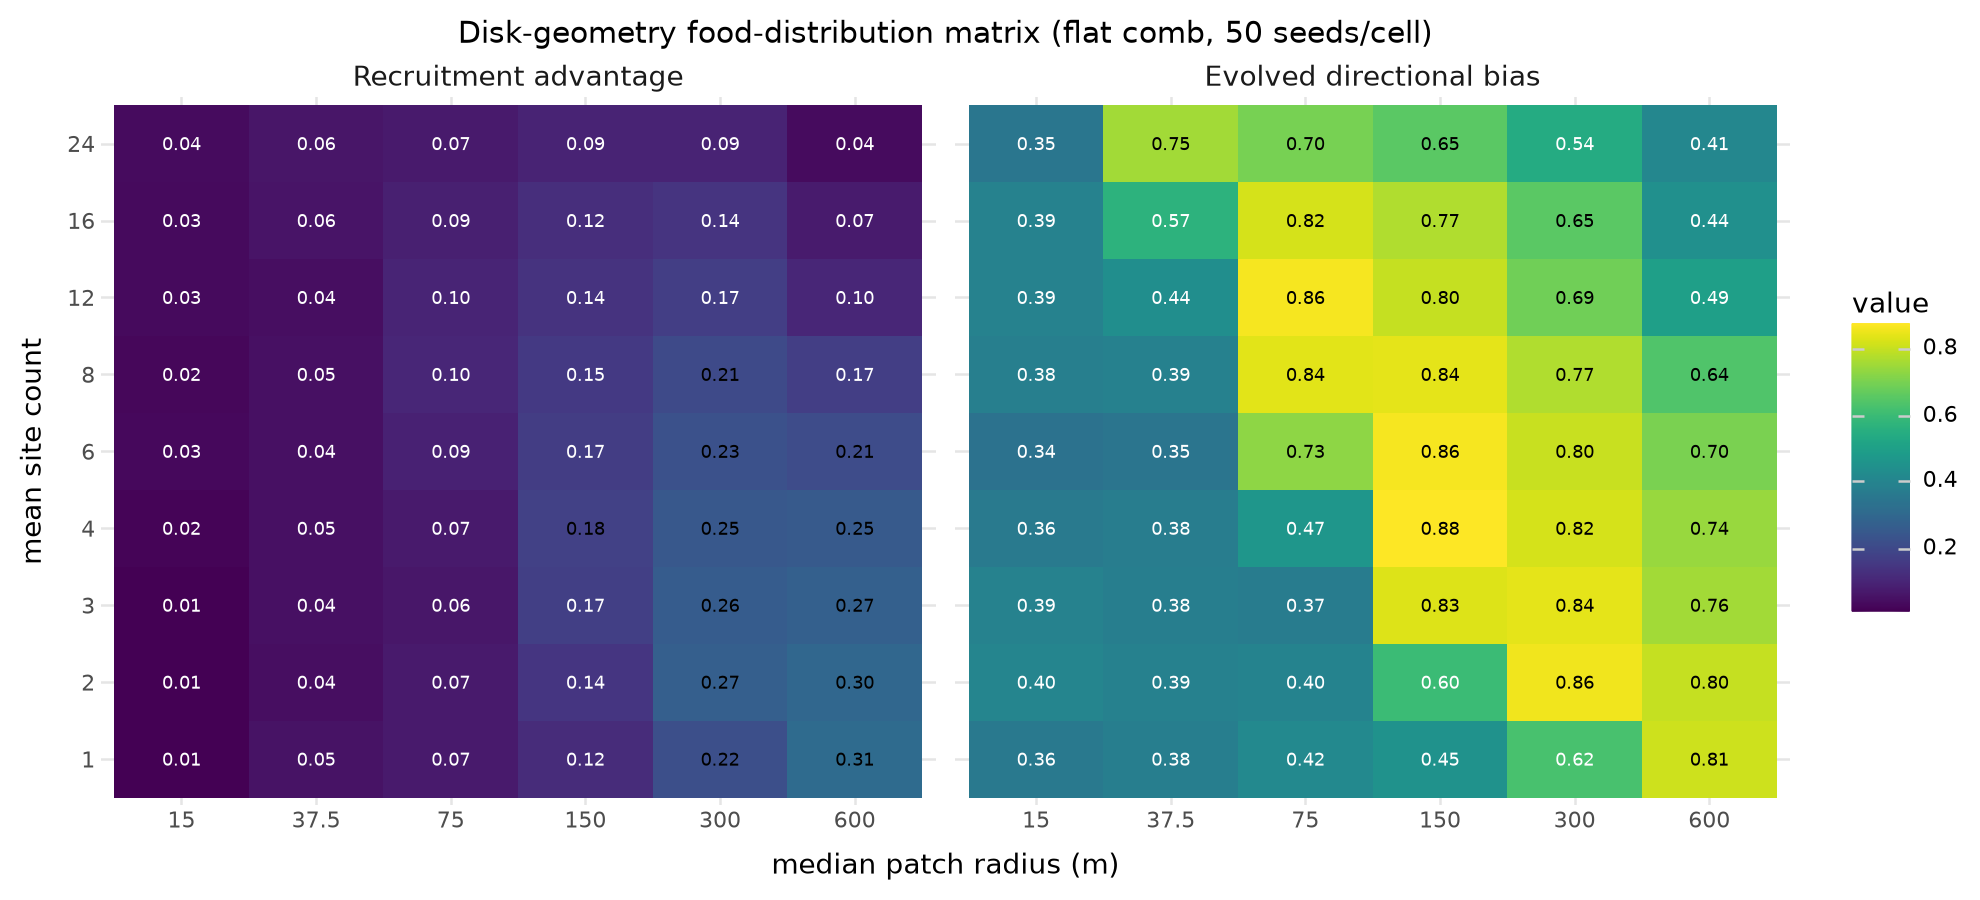
\includegraphics[width=0.9\textwidth]{figures/food_distribution_disk_grid.png}
  \caption{Evolved \trait{directional bias} (left) and recruitment advantage (right) on a
    flat comb across the grid of Poisson mean site count against median patch
    radius, $50$ seeds per cell. Recruitment advantage is the follower--searcher
    success difference, and shading is normalized within each panel. The bias
    traces a diagonal band whose patch-size threshold falls as patches grow more
    numerous, whereas the recruitment advantage instead peaks for few, large
    patches and erodes toward both small and abundant food.}
  \label{fig:food-grid}
\end{figure}
\subsection{Evolution of the gravity code}
\label{sec:results-transition}

\paragraph{Parameter search.}
Stable vertical-gravity transitions are common under both decodes, and unproject is
slightly broader (\Cref{tab:optuna-stability}). Both searches concentrate their
strongly stable trials in much the same region: abundant, large, reachable food
paired with a strong tilt incentive and a high mutation scale
(\Cref{tab:optuna-region}). The main difference is that unproject tolerates
food at longer range (median maximum distance $5.25$ km against flatten's $3.25$ km).
The sender--receiver correlation $\rho$ is not
decisive, its stable range spanning almost the whole $[0,1]$ axis under both
decodes, and mean foraging success across the strongly stable trials is only $0.27$
in each, so the transition needs a reliably communicable ecology rather than an
abundant one.

\begin{table}
  \centering
  \begin{tabular}{lrr}
    \toprule
    Outcome & Flatten trials & Unproject trials \\
    \midrule
    Stable in all $10$ seeds & $14$ & $24$ \\
    Stable in $\ge 8$ seeds   & $123$ & $132$ \\
    Stable in $\ge 5$ seeds   & $312$ & $338$ \\
    Stable in $\ge 1$ seed    & $611$ & $641$ \\
    No stable seed            & $413$ & $383$ \\
    \bottomrule
  \end{tabular}
  \caption{Stability counts over the $1024$ Optuna trials (ten seeds each) under
    each decode.}
  \label{tab:optuna-stability}
\end{table}

\begin{table}
  \centering
  \small
  \begin{tabular}{lrlrl}
    \toprule
    & \multicolumn{2}{c}{Flatten} & \multicolumn{2}{c}{Unproject} \\
    \cmidrule(lr){2-3}\cmidrule(lr){4-5}
    Parameter & Median & 10th--90th & Median & 10th--90th \\
    \midrule
    Food-site count (Poisson mean) & $8$    & $5$--$8$   & $8$    & $6$--$8$ \\
    Patch radius (m)               & $210$  & $165$--$345$ & $225$  & $150$--$360$ \\
    Patch capacity                 & $7$    & $2$--$8$   & $7$    & $3$--$9$ \\
    Vertical-comb benefit $B$      & $0.56$ & $0.50$--$0.56$ & $0.56$ & $0.50$--$0.56$ \\
    Max food distance (km)         & $3.25$ & $3.25$--$5.25$ & $5.25$ & $3.5$--$5.25$ \\
    Travel cost per km             & $0.025$ & $0.010$--$0.025$ & $0.018$ & $0.010$--$0.022$ \\
    Mutation scale $\sigma_m$      & $0.110$ & $0.090$--$0.110$ & $0.110$ & $0.110$--$0.130$ \\
    Correlation $\rho$             & $0.4$   & $0.0$--$0.9$ & $0.4$   & $0.0$--$1.0$ \\
    \bottomrule
  \end{tabular}
  \caption{Parameter distribution of the strongly stable trials (eight or more of
    ten stable seeds) under each decode.}
  \label{tab:optuna-region}
\end{table}

\paragraph{Held-out validation.}
The top five distinct candidates from each search, rerun on $100$ held-out seeds
($200$--$299$), all produced frequent stable transitions and no collapse events;
stable rates ran $80$--$91$ of $100$ for flatten and $82$--$92$ for unproject. The
strongest candidate of each decode (\Cref{tab:validation}) lands on very similar
held-out rates and on overlapping ecologies: large patches, short-to-moderate
distances, low travel cost, high benefit.

\begin{table}
  \centering
  \small
  \begin{tabular}{llrrrrrrrrr}
    \toprule
    Decode & Cand. & Sites & Rad. (m) & Cap. & $B$ & Dist. (km) & Travel/km & $\sigma_m$ & Stable & $t_f$ \\
    \midrule
    flatten   & 729 & $5$ & $315$ & $4$  & $0.56$ & $3.25$ & $0.017$ & $0.070$ & $91/100$ & $0.845$ \\
    unproject & 541 & $7$ & $315$ & $12$ & $0.60$ & $4.75$ & $0.010$ & $0.090$ & $92/100$ & $0.848$ \\
    \bottomrule
  \end{tabular}
  \caption{Strongest validated candidate per decode over $100$ held-out seeds;
    $t_f$ is final mean \trait{comb tilt}. Both reach foraging success ${\approx}0.35$,
    higher than the $0.27$ mean across all strongly stable search trials, as
    expected for the single strongest candidate of each decode.}
  \label{tab:validation}
\end{table}

\paragraph{One-parameter sensitivity.}
A one-parameter sweep around each validated baseline identifies the mutation scale
as the sharpest boundary (\Cref{fig:sensitivity-flatten,fig:sensitivity-unproject}):
lowering it collapses the
transition (flatten falls from $91/100$ to $49/100$ at $\sigma_m = 0.05$; unproject
to $16/100$ at $0.04$), while the validated $\sigma_m$ of $0.07$--$0.09$ sits on the
plateau. The sharpest \emph{ecological} boundary is food-site count under flatten
($46/100$ at a Poisson mean of two, rising to $87/100$ at seven); unproject is more
robust to count. Vertical-comb benefit and correlation are monotone and moderate,
and patch radius, capacity, distance, and travel cost stay within a narrow band.

\begin{figure}
  \centering
  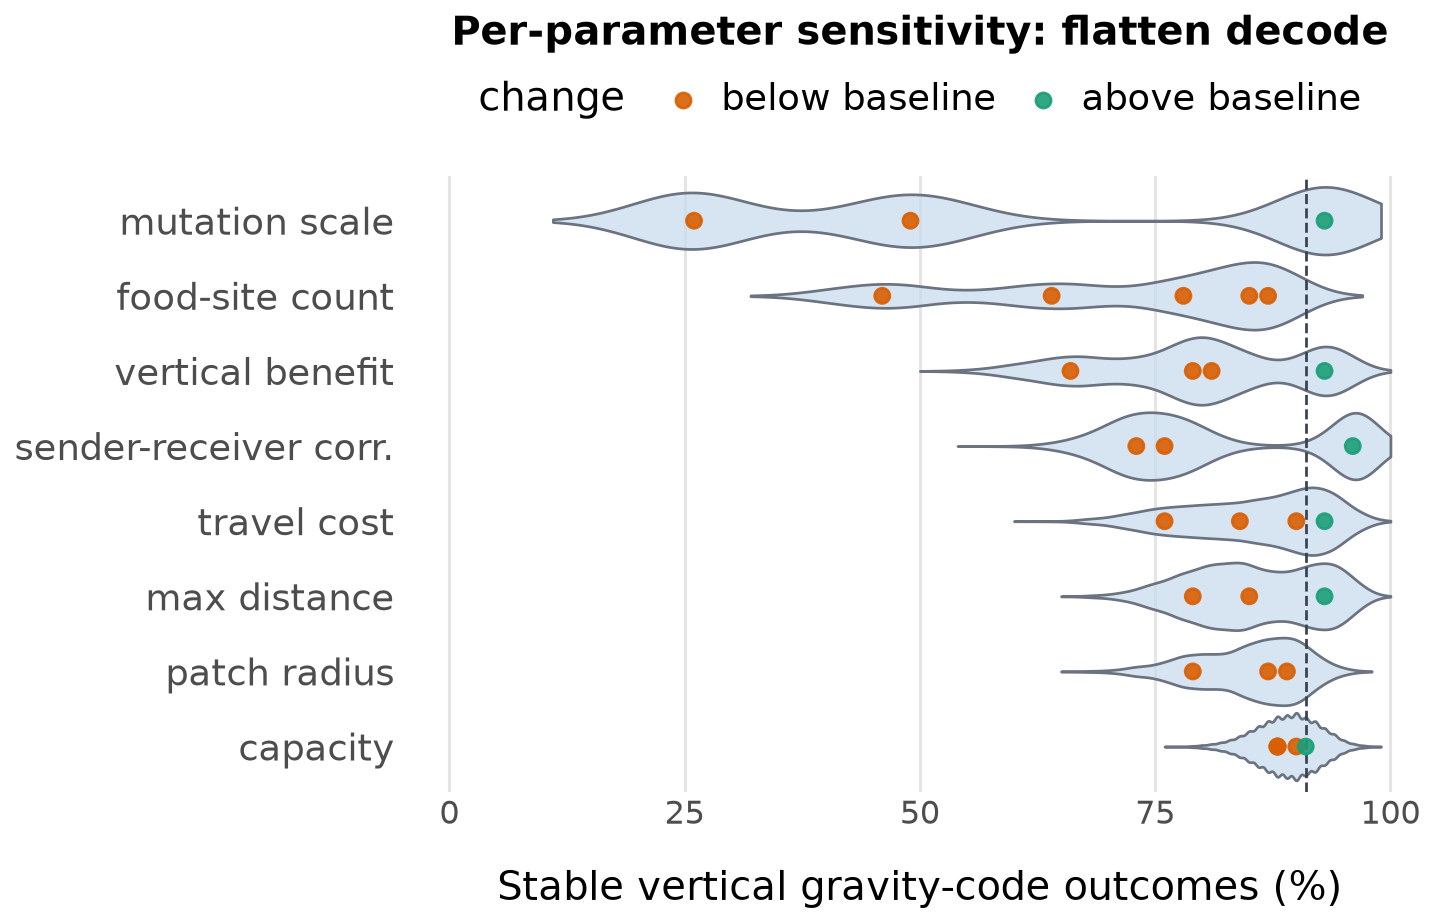
\includegraphics[width=0.82\textwidth]{figures/food_transition_disk_sensitivity_ridge_flatten.png}
  \caption{One-parameter sensitivity of the flatten decode. Each parameter's violin
    is a kernel density over seed-bootstrap stable-rate draws pooled across that
    parameter's swept values ($100$ held-out seeds per value), so a lobe's position
    is a swept value's rate and its width that value's sampling uncertainty; dots
    mark the per-value rates (orange below, green above baseline) and the dashed line
    the baseline. Parameters are sorted by worst-case drop (shared order and x-range
    with \Cref{fig:sensitivity-unproject}). Mutation scale is the widest,
    most collapse-prone lever and food-site count the sharpest ecological one, while
    patch radius and capacity stay tightly at baseline.}
  \label{fig:sensitivity-flatten}
\end{figure}

\begin{figure}
  \centering
  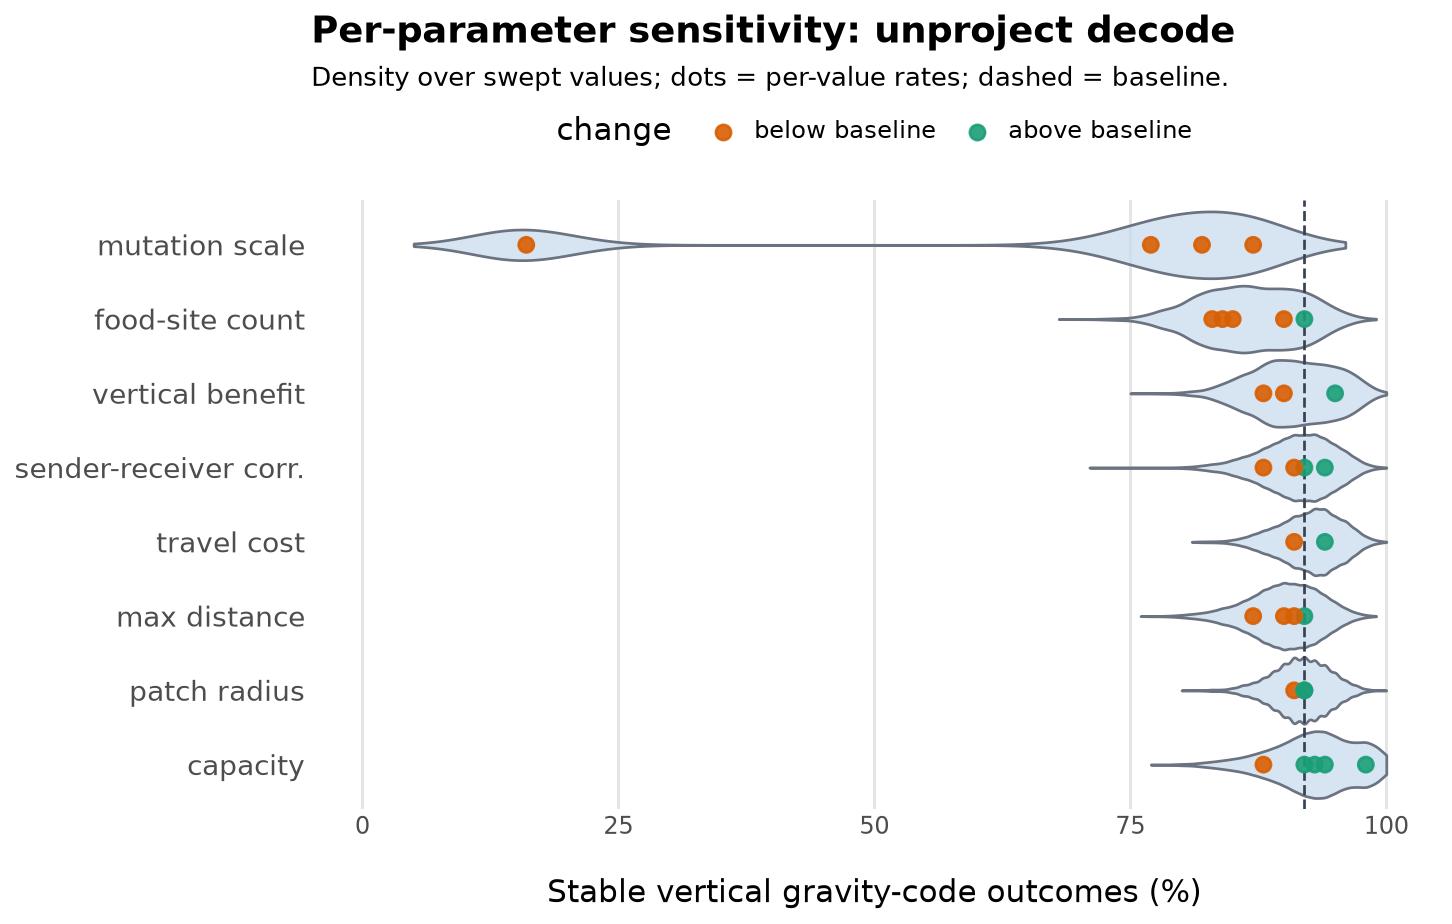
\includegraphics[width=0.82\textwidth]{figures/food_transition_disk_sensitivity_ridge_unproject.png}
  \caption{One-parameter sensitivity of the unproject decode, drawn as in
    \Cref{fig:sensitivity-flatten} and sharing its parameter order and x-range.
    Mutation scale is again the sharpest boundary (a lone collapse at
    $\sigma_m = 0.04$), but every other parameter stays tightly at baseline; in
    particular, unproject is markedly more robust to food-site count than flatten.}
  \label{fig:sensitivity-unproject}
\end{figure}

\paragraph{Evolutionary-parameter interaction.}
Fixing each decode's validated ecology and sweeping $B$, $\sigma_m$, and $\rho$
across the search range, stable rate falls steeply with benefit: robust near the
validated $B\approx0.56$--$0.60$, already marginal by $B=0.30$, and collapsing at
the search floor $B=0.10$, with unproject again slightly more robust than flatten
(\Cref{fig:interaction}). Within each benefit panel the rate rises with mutation
scale and with correlation, and the best cells pair a high mutation scale
($0.09$--$0.11$) with moderate-to-high correlation, so higher mutation and
correlation only partly compensate for weaker architectural benefit. This
compensation from correlation is concentrated in the low-mutation regime: at the
smallest mutation scale, raising the correlation from $0$ to $0.9$ roughly
doubles the stable rate, whereas at the highest mutation scale its effect is much
weaker, and slightly negative under unproject.

\begin{figure}
  \centering
  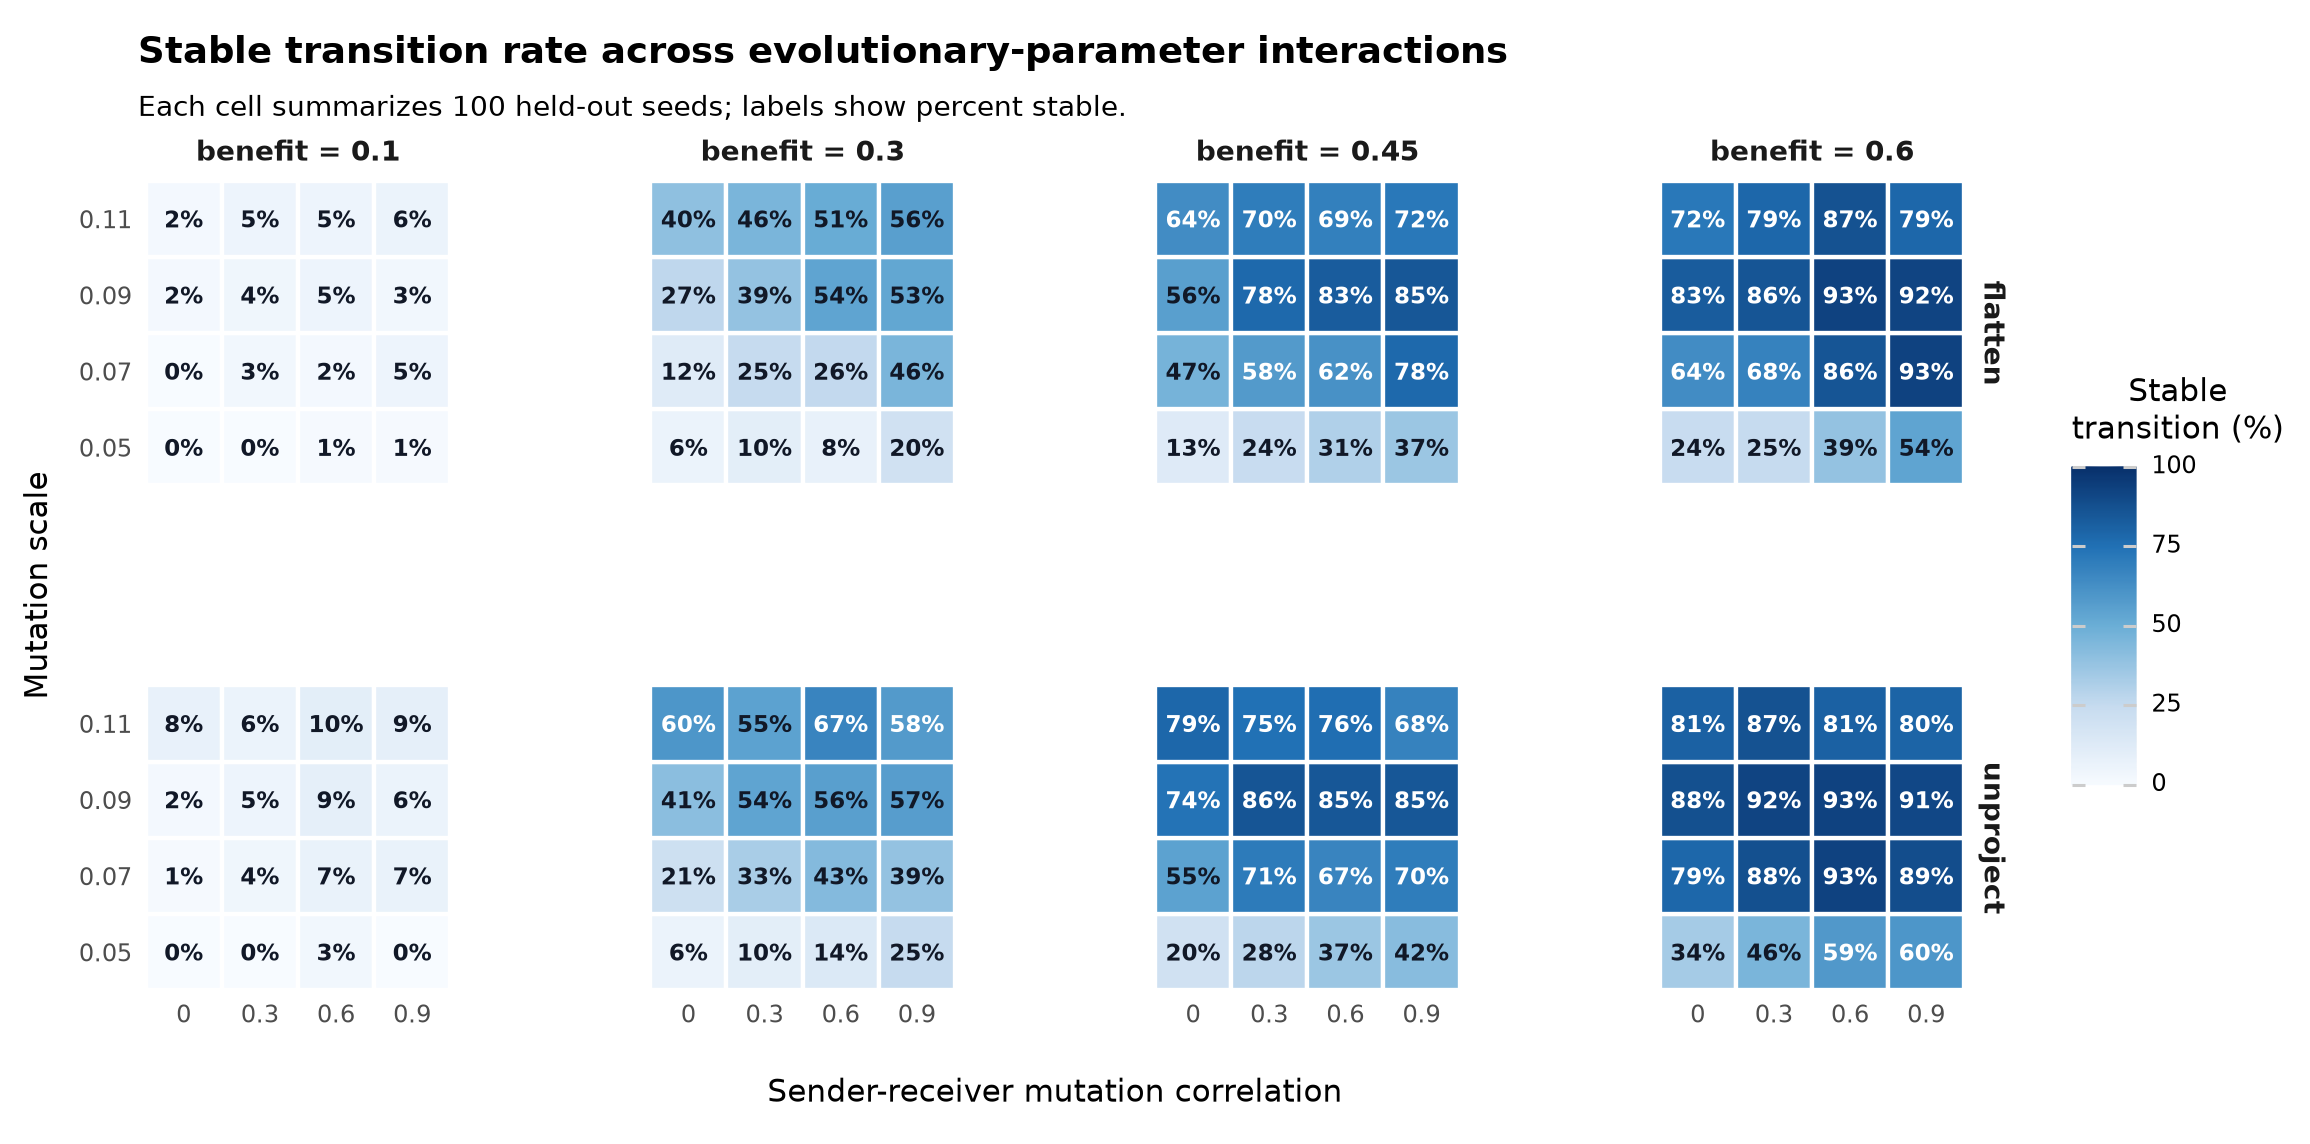
\includegraphics[width=\textwidth]{figures/food_transition_disk_interaction_heatmap.png}
  \caption{Stable transition rate across the evolutionary-parameter interaction
    grid, holding each decode's validated ecology fixed. Benefit is swept across
    the full search range ($0.10$--$0.60$) as a generic gradient rather than
    through the validated operating points (flatten $B{=}0.56$, unproject
    $B{=}0.60$). Tiles cross the sender--receiver mutation correlation $\rho$
    against the mutation scale $\sigma_m$, faceted by decode (rows) and
    vertical-comb benefit $B$ (columns); each cell summarizes $100$ held-out
    seeds, and its label is the percentage of seeds with a stable transition.
    Stable rate rises with benefit, mutation scale, and correlation, and
    unproject clears a broader region than flatten at every benefit.}
  \label{fig:interaction}
\end{figure}

\section{Discussion and Conclusion}
\label{sec:discussion}

Our finding that the transition to the gravity-referenced code can proceed without
a breakdown of communication, under suitable ecological and evolutionary
conditions, complements the mechanistic proposal of \citet{10.1242/jeb.142778}: if
the underlying heading representation is indifferent to the spatial reference
frame, then the principal barrier to changing the code is not the neural machinery
but the ecological and coordination conditions that our model isolates.
\section{Limitations}
\label{sec:limitations}

\bibliographystyle{apalike}
\bibliography{biblio}

\end{document}
